\documentclass[hyperref={pdftex,pdfpagemode=none,pdfstartview=FitH},10pt,aspectratio=43]{beamer}
\usepackage[english]{babel}
\usepackage{times}
\usepackage{amsmath,amssymb,bm}
\usepackage{subfigure,graphicx}
\usepackage{multirow,booktabs,diagbox,makecell}
\usepackage{tikz}
\usepackage{cases,booktabs}
\usetikzlibrary{arrows.meta}
\usetikzlibrary{shapes.arrows}
\usepackage{siunitx}
\usepackage{hyperref}
\usepackage{xcolor}

\newcommand{\SO}[1]{\ensuremath{\mathrm{SO}(#1)}}
\newcommand{\SE}[1]{\ensuremath{\mathrm{SE}(#1)}}
\newcommand{\so}[1]{\ensuremath{\mathfrak{so}(#1)}}
\newcommand{\Sph}{\ensuremath{\mathbb{S}}}
\newcommand{\norm}[1]{\ensuremath{\left\| #1 \right\|}}
\newcommand{\tr}[1]{\ensuremath{\mathrm{tr}\left( #1 \right)}}
\newcommand{\etr}[1]{\ensuremath{\mathrm{etr}\left( #1 \right)}}
\newcommand{\expect}[1]{\ensuremath{\mathrm{E}\left[ #1 \right]}}
\newcommand{\expectbar}[1]{\ensuremath{\bar{\mathrm{E}}\left[ #1 \right]}}
\newcommand{\cov}[2]{\ensuremath{\mathrm{cov}\left( #1, #2 \right)}}
\newcommand{\covbar}[2]{\ensuremath{\overline{\mathrm{cov}}\left( #1, #2 \right)}}
\newcommand{\expb}[1]{\ensuremath{\exp\left\{ #1 \right\}}}
\newcommand{\diff}{\ensuremath{\mathrm{d}}}
\newcommand{\diag}{\ensuremath{\mathrm{diag}}}

\makeatletter
\newcommand\approxsim{\mathchoice
	{\@approxsim {\displaystyle}      {1ex} }
	{\@approxsim {\textstyle}         {1ex} }
	{\@approxsim {\scriptstyle}       {.7ex}}
	{\@approxsim {\scriptscriptstyle} {.5ex}}}
\newcommand\@approxsim[2]{%
	\mathrel{%
		\ooalign{%
			$\m@th#1\sim$\cr
			\hidewidth$\m@th#1.$\hidewidth\cr
			\hidewidth\raise #2 \hbox{$\m@th#1.$}\hidewidth\cr
		}%
	}%
}
\makeatother

\setbeamerfont{footnote mark}{size=\tiny}

\definecolor{RoyalBlue}{rgb}{0.25,0.41,0.88}
\def\Emph{\textcolor{RoyalBlue}}

\definecolor{mygray}{gray}{0.9}
\definecolor{tmp}{rgb}{0.804,0.941,1.0}
%\setbeamercolor{numerical}{fg=black,bg=tmp}
\setbeamercolor{exact}{fg=black,bg=red}
\setbeamercolor{numerical}{fg=black,bg=mygray}

\mode<presentation> {
  \usetheme{Berkeley}
  \usefonttheme{serif}
  \setbeamercovered{transparent}
}

\setbeamertemplate{footline}%{split theme}
{%
  \leavevmode%
  \hbox{\begin{beamercolorbox}[wd=.5\paperwidth,ht=2.5ex,dp=1.125ex,leftskip=.3cm,rightskip=.3cm plus1fill]{author in head/foot}%
    \usebeamerfont{author in head/foot}\insertshorttitle
  \end{beamercolorbox}%
  \begin{beamercolorbox}[wd=.5\paperwidth,ht=2.5ex,dp=1.125ex,leftskip=.3cm plus1fill,rightskip=.3cm]{title in head/foot}%
    \usebeamerfont{title in
    head/foot}\insertframenumber/\inserttotalframenumber
  \end{beamercolorbox}}%
  \vskip0pt%
} \setbeamercolor{box}{fg=black,bg=yellow}

\title[]{Geometric Formulation of Uncertainties and Estimation for Three-Dimensional Rotations}

\author[]{Weixin Wang \\ Advisor: Prof. Taeyoung Lee}

\institute[GWU]{\footnotesize\selectfont
Department of Mechanical and Aerospace Engineering\\
George Washington University, Washington DC\\$ $\\}

\date{July 21, 2022}

\graphicspath{{./Figs/},{../figures/},{../figures/observability/}}

\newenvironment<>{varblock}[2][12cm]{
    \begin{center}
      \begin{minipage}{#1}
        \setlength{\textwidth}{#1}
          \begin{actionenv}#3
            \def\insertblocktitle{#2}
            \par
            \usebeamertemplate{block begin}}
  {\par
      \usebeamertemplate{block end}
    \end{actionenv}
  \end{minipage}
\end{center}}

\newenvironment<>{varblock2}[2][0.7\textwidth]{
          \begin{actionenv}#3
            \def\insertblocktitle{#2}
            \par
            \usebeamertemplate{block begin}}
  {\par
      \usebeamertemplate{block end}
    \end{actionenv}
}

\DeclareMathOperator*{\argmin}{arg\,min}
\DeclareMathOperator*{\argmax}{arg\,max}

%%%%%%%%%%%%%%%%%%%%%%%%%%%%%%%%%%%%%%%%%%%%%%%%%%%%%%%%%%%%

\begin{document}

\setcounter{framenumber}{-1}
\begin{frame}
	\titlepage
\end{frame}

\begin{frame}
	\frametitle{Overview}
	\tableofcontents
\end{frame}

\section{Motivation}

\begin{frame}
	\frametitle{Attitude Estimation in Engineering}
	
	\begin{itemize}
		\item 3D Rigid Body Attitude
		\begin{itemize}
			\item The orientation of a reference frame fixed to the rigid body.
			\item The space of 3D attitude: three dimensional special orthogonal group.
			
			\centerline{
				\begin{beamercolorbox}[wd=10cm,sep=0.0cm,center,rounded=true,shadow=true]{numerical}
					\small
					\vspace{-0.3cm}
					\begin{equation*}
						\SO{3} = \{R\in\mathbb{R}^{3\times 3} \,|\, RR^T = I_{3\times 3},\, \det(R) = 1\}.
					\end{equation*}
					\vspace{-0.5cm}
				\end{beamercolorbox}
			}
			
			\item Rotation matrix $R\in\SO{3}$: transform the coordinates of a vector from the \Emph{body-fixed frame} $x^B$ to \Emph{inertial frame} $x^I$.
			
			\centerline{
				\begin{beamercolorbox}[wd=10cm,sep=0.0cm,center,rounded=true,shadow=true]{numerical}
					\small
					\vspace{-0.3cm}
					\begin{equation*}
						x^I = Rx^B
					\end{equation*}
					\vspace{-0.5cm}
				\end{beamercolorbox}
			}
		\end{itemize}
	
		\vspace{0.3cm}
		\item Applications in Engineering
		\begin{itemize}
			\item Alignment of two satellites: laser communication.
			\item Attitude control for UAVs.
			\item Inertial navigation.
		\end{itemize}
	\end{itemize}
\end{frame}

\begin{frame}
	\frametitle{Uncertainty for 3D Attitude}
	
	\begin{itemize}
		\item State Estimation of a Dynamical System
		\begin{itemize}
			\item Uncertainty Propagation: propagete the mean and covariance matrix of the state through the kinematic equations.
			\item Measurement Update: use new measurements to correct propagation errors.
			\item Covariance matrices are used to weigh the propagation and measurement noises.
		\end{itemize}
	
		\vspace{0.3cm}
		\item What is Covariance Matrix for 3D Rotation?
		\begin{itemize}
			\item Covariance for lower dimensional parameterizations:
			\begin{itemize}
				\item Three dimensional: Euler angles, (modified) Rodrigues parameters, etc.
				\item Four dimensional: Unit quaternions.
			\end{itemize}
		
			\item Problems with three dimensional parameterizations:
			\begin{itemize}
				\item \Emph{Singularities}: such as gimbal lock for Euler angles.
				\item The Lebesgue measure on $\mathbb{R}^3$ is no longer uniform when transformed to $\SO{3}$.
			\end{itemize}
		
			\item Problems with quaternions:
			\begin{itemize}
				\item The \Emph{unit norm constraint} makes the covariance matrix singular.
			\end{itemize}
		\end{itemize}
	\end{itemize}
\end{frame}

\begin{frame}
	\frametitle{Multiplicative Extended Kalman Filter}
	\begin{itemize}
		\item Covariance Matrix for \Emph{Attitude Error}
		
		\centerline{
			\begin{beamercolorbox}[wd=10cm,sep=0.0cm,center,rounded=true,shadow=true]{numerical}
				\small
				\vspace{-0.3cm}
				\begin{equation*}
					q_t = q \otimes q\{\delta v\}.
				\end{equation*}
				\vspace{-0.5cm}
			\end{beamercolorbox}
		}
		
		\begin{itemize}
			\item $q_t,q\in\Sph^3$: true and estimated attitude represented by unit quaternions.
			\item $q\{\delta v\} \in \Sph^3$: error attitude expressed as a rotation vector $\delta v\in\mathbb{R}^3$.
			\item $\delta v \sim \mathcal{N}(0,\Sigma)$, where $\Sigma\in\mathbb{R}^{3\times 3}$ is the covariance matrix, representing the uncertainty of the attitude.
			\begin{itemize}
				\item $\delta v$ is three dimensional.
				\item $\delta v$ is usually small, so singularity is avoided.
			\end{itemize}
		\end{itemize}
	
		\vspace{0.3cm}
		\item Multiplicative Extended Kalman Filter
		\begin{itemize}
			\item Using Gaussian distribution to model the uncertainty of attitude error.
			\item Problems: \Emph{not suitable for large uncertainty}
			\begin{itemize}
				\item Linearization error.
				\item Wrapping error.
			\end{itemize}
		\end{itemize}
	\end{itemize}
\end{frame}

\begin{frame}
	\frametitle{Problems for Gaussian Distribution}
	
	\begin{itemize}
		\item Attitude Error is in the \Emph{Tangent Space} of $\SO{3}$.
		
		\vspace{0.4cm}
		\item Problems: not suitable for large uncertainty
		\begin{itemize}
			\item Inherent \Emph{non-linearity}: $\SO{3}$ is a curved manifold.
			\item \Emph{Wrapping errors} for cyclic tangent space.
		\end{itemize}
		
		\vspace{-0.1cm}
	
		\centerline{
			\begin{tikzpicture}
				\node[opacity=1.0,outer sep=0pt,inner sep=0pt] at (0,0) {\includegraphics[scale=0.4]{circle_density_edited}};
				\node[opacity=1.0,outer sep=0pt,inner sep=0pt] at (5.2,-0.2) {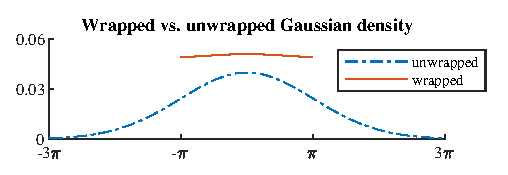
\includegraphics[scale=0.7]{wrapping}};
			\end{tikzpicture}
		}
	
		\pause
		\item A probability distribution \Emph{directly defined on $\SO{3}$} could avoid these issues.
	\end{itemize}
\end{frame}

\section{Matrix Fisher Distribution}

\begin{frame}
	\frametitle{Matrix Fisher Distribuiton}
	
	\begin{itemize}
		\item Matrix Fisher Distribution: Defined on $\SO{3}$
		\begin{itemize}
			\item Construction: condition a Gaussian distribution from $\mathbb{R}^9$ to $\SO{3}$.
			\item Density function for $R\sim\mathcal{M}(F)$:
			
			\centerline{
				\begin{beamercolorbox}[wd=10cm,sep=0.0cm,center,rounded=true,shadow=true]{numerical}
					\small
					\vspace{-0.3cm}
					\begin{equation*}
						p(R) = \frac{1}{c(F)} \expb{\tr{FR^T}}.
					\end{equation*}
					\vspace{-0.4cm}
				\end{beamercolorbox}
			}
		
			\begin{itemize}
				\item $F\in\mathbb{R}^{3\times 3}$ is the parameter, $c(F)\in\mathbb{R}$ is the normalizing constant.
			\end{itemize}
		\end{itemize}
	
		\vspace{0.2cm}
		\item Bingham Distribution: Defined on $\Sph^3$
		\begin{itemize}
			\item \Emph{Equivalent to the matrix Fisher distribution} under the homomorphism from $\SO{3}$ to $\Sph^3$.
		\end{itemize}
	\end{itemize}
	
	\vspace{0.2cm}
	\only<1>{\centerline{
			\begin{tikzpicture}
				\node[opacity=1,outer sep=0pt,inner sep=0pt] at (0,0) {\includegraphics[scale=0.2]{MFDensity1}};
				\node[opacity=1,outer sep=0pt,inner sep=0pt] at (3,0) {\includegraphics[scale=0.2]{MFDensity2}};
				\node[opacity=1,outer sep=0pt,inner sep=0pt] at (6,0) {\includegraphics[scale=0.2]{MFDensity3}};
			\end{tikzpicture}
	}}
\end{frame}

\begin{frame}
	\frametitle{Properties}
	
	\begin{itemize}
		\item Shape of the Density Function
		\begin{itemize}
			\item proper singular value decomposition (pSVD) of the parameter: $F = USV^T$.
			\item \Emph{Mean attitude}: $M = UV^T$ (uni-modal).
			\item \Emph{Principal axes}:
			\begin{itemize}
				\item Columns of $U$ in the inertial frame.
				\item Columns of $V$ in the body-fixed frame of the mean attitude $M$.
			\end{itemize}
			\item \Emph{Dispersion}: $s_i+s_j$ specifies the dispersion along the $k$-th principal axis, for $i\neq j\neq k$.
			\item Analogous to a Gaussian distribution.
		\end{itemize}
	
		\vspace{0.2cm}
		\item Maximum Likelihood Estimation (MLE) for Parameters
		\begin{itemize}
			\item Moments
			
			\centerline{
				\begin{beamercolorbox}[wd=10cm,sep=0.0cm,center,rounded=true,shadow=true]{numerical}
					\small
					\vspace{-0.3cm}
					\begin{equation*}
						\expect{R} = UDV^T, \qquad \qquad d_i = \frac{1}{c(S)} \frac{\partial c(S)}{\partial s_i}.
					\end{equation*}
					\vspace{-0.4cm}
				\end{beamercolorbox}
			}
		
			\item MLE for $U,V\in\SO{3}$: the pSVD of $\expect{R} = USV^T$.
			\item MLE for $S$: solving $d_i = \frac{1}{c(S)} \frac{\partial c(S)}{\partial s_i}$ from $D$.
		\end{itemize}
	\end{itemize}
\end{frame}

\begin{frame}
	\frametitle{Central Moments}
	\begin{itemize}
		\item Motivation
		\begin{itemize}
			\item Designing Bayesian filters using matrix Fisher distribution sometimes needs to evaluate its higher order moments.
		\end{itemize}

		\vspace{0.2cm}
		\item Central Moments for Matrix Fisher Distribution: $Q = U^TRV$
		
		\centerline{
			\begin{beamercolorbox}[wd=10cm,sep=0.0cm,center,rounded=true,shadow=true]{numerical}
				\small
				\vspace{-0.3cm}
				\begin{equation*}
					\expect{Q_{i_1j_1}\cdots Q_{i_nj_n}} = \frac{1}{c(S)} \left. \frac{\partial c(S+T)}{\partial T_{i_1j_1} \cdots \partial T_{i_nj_n}} \right|_{T = 0}.
				\end{equation*}
				\vspace{-0.4cm}
			\end{beamercolorbox}
		}
	
		\begin{itemize}
			\item $\expect{Q_{i_1j_1}\cdots Q_{i_nj_n}} = 0$ if $\{i_k,j_k\}_{k=1}^n$ has odd number of 1, 2, or 3.
			\item $\expect{Q_{i_1j_1}\cdots Q_{i_nj_n}} = \expect{Q_{j_1i_1} \cdots Q_{j_ni_n}}$.
		\end{itemize}
	
		\vspace{0.2cm}
		\item Computation
		\begin{itemize}
			\item $\expect{Q_{i_1j_1}\cdots Q_{i_nj_n}}$ is a linear combination of the derivatives of $c(S)$ up to $n$-th order.
			\item The coefficients and derivatives of $c(S)$ can be calculated recursively.
			\item The recursion starts from $c(S)$ and its first order derivatives $\frac{\partial c(S)}{\partial s_i}$.
		\end{itemize}
	\end{itemize}
\end{frame}

\begin{frame}
	\frametitle{Highly Concentrated Approximations}
	
	\begin{itemize}
		\item Motivation
		\begin{itemize}
			\item Evaluating the normalizing constant $c(S)$ and its derivatives is hard.
			\item The MLE $d_i = \frac{1}{c(S)} \frac{\partial c(S)}{\partial s_i}$ is very hard to solve.
		\end{itemize}
	
		\vspace{0.2cm}
		\only<1>{
			\item Highly Concentrated in Three Degrees of Freedom
			\begin{theorem}
				Let $R\sim\mathcal{M}(F)$, where $F=USV^T$ is the pSVD of $F$.
				Suppose $s_2+s_3\gg 0$.
				Let $Q = U^TRV = \exp\left(\hat{\eta}\right)$, then \Emph{$\eta \approxsim \mathcal{N}\big( 0,\allowbreak (\tr{S}I_{3\times 3}-S)^{-1} \big)$}.
			\end{theorem}
		
			\begin{itemize}
				\item The matrix Fisher distribution is approximated by a Gaussian distribution in $\mathbb{R}^3$.
			\end{itemize}
		}
	
		\only<2>{
			\item Highly Concentrated in Three Degrees of Freedom
			
			\begin{itemize}
				\item Approximations of $c(S)$ and its derivatives ($i\neq j\neq k$):
				
				\centerline{
					\begin{beamercolorbox}[wd=10cm,sep=0.0cm,center,rounded=true,shadow=true]{numerical}
						\small
						\vspace{-0.3cm}
						\begin{align*}
							c(S) &\approx \frac{\etr{S}}{\sqrt{8\pi(s_1+s_2)(s_1+s_3)(s_2+s_3)}} \label{eqn:MF-normalizing-approx1} \\
							\frac{1}{c(S)} \frac{\partial c(S)}{\partial s_i} &\approx 1 - \frac{1}{2}\left( \frac{1}{s_i+s_j} + \frac{1}{s_i+s_k} \right), \label{eqn:MF-S2D-approx1}
						\end{align*}
						\vspace{-0.4cm}
					\end{beamercolorbox}
				}
			\end{itemize}
		}
	
		\only<3>{
			\item Highly Concentrated in Two Degrees of Freedom
			\begin{theorem}
				Let $R\sim\mathcal{M}(F)$, where $F=USV^T$ is the pSVD of $F$.
				Suppose $s_1+s_3\gg s_2+s_3 \geq 0$.
				Let $Q = U^TRV = \exp\left(\hat{\eta}\right) \exp\left(\hat{\eta}'\right)$, where $\eta = [0, \eta_2, \eta_3]^T$, and $\eta' = [\eta_1, 0, 0]^T$.
				Then \Emph{$\eta_3 \approxsim \mathcal{VM}(0,s_2+s_3)$}, and \Emph{$[\eta_2, \eta_3]^T  \approxsim \mathcal{N}\left( 0, \diag\left( \tfrac{1}{s_1+s_3}, \tfrac{1}{s_1+s_2} \right) \right)$}, and they are approximately independent.
			\end{theorem}
		
			\begin{itemize}
				\item The matrix Fisher distribution is approximated by a combination of Gaussian distribution in $\mathbb{R}^2$, and a von Mises distribution on $\Sph^1$.
			\end{itemize}
		}
	
		\only<4>{
			\item Highly Concentrated in Two Degrees of Freedom
			\begin{itemize}
				\item Approximations of $c(S)$ and its derivatives ($j\in\{2,3\}$):
				
				\centerline{
					\begin{beamercolorbox}[wd=10cm,sep=0.0cm,center,rounded=true,shadow=true]{numerical}
						\small
						\vspace{-0.3cm}
						\begin{align*}
							c(S) &\approx \frac{\exp(s_1)I_0(s_2+s_3)}{2\sqrt{(s_1+s_2)(s_1+s_3)}}, \label{eqn:MF-normalizing-approx2} \\
							\frac{1}{c(S)}\frac{\partial c(S)}{\partial s_1} &\approx 1 - \frac{1}{2}\left( \frac{1}{s_1+s_2} + \frac{1}{s_1+s_3} \right), \label{eqn:MF-S2D-approx2-1} \\
							\frac{1}{c(S)}\frac{\partial c(S)}{\partial s_j} &\approx \frac{I_1(s_2+s_3)}{I_0(s_2+s_3)} - \frac{1}{2}\frac{1}{s_1+s_j}, \label{eqn:MF-S2D-approx2-2}
						\end{align*}
						\vspace{-0.4cm}
					\end{beamercolorbox}
				}
			\end{itemize}
		}
	\end{itemize}
\end{frame}

\section{Matrix Fisher--Gaussian Distribution}

\begin{frame}
	\frametitle{Correlation Between $\SO{3}$ and $\mathbb{R}^n$}
	
	\begin{itemize}
		\item Examples
		\begin{itemize}
			\item Attitude estimation: correlation between attitude and gyroscope bias.
			\item Inertial navigation: correlation between attitude and position.
			\item SLAM: correlation between attitude and landmark locations.
		\end{itemize}
	
		\vspace{0.2cm}
		\item Existing Models
		\begin{itemize}
			\item In Markley 2006\footnote{\tiny F.~L. Markley, ``Attitude filtering on $\mathrm{SO}(3)$,'' \emph{The Journal of the Astronautical Sciences}, vol.~54, no. 3-4, pp. 391--413, 2006.}, the matrix Fisher distribution on $\SO{3}$ is combined with Gaussian distribution in $\mathbb{R}^n$.
			
			\item In Darling 2016\footnote{\tiny J.~E. Darling and K.~J. DeMars, ``Uncertainty propagation of correlated quaternion and {E}uclidean states using the {G}auss-{B}ingham density,'' \emph{Journal of Advances in Information Fusion}, vol.~11, no.~2, pp. 1--20, 2016}, the Bingham distribution on $\Sph^3$ is combined with Gaussian distribution in $\mathbb{R}^n$.
			
			\item Problems:
			\begin{itemize}
				\item These models do not have a generic geometric construction.
				\item Their MLEs are complicated and need numerical optimizations, so they are \Emph{not suitable for real time implementations}.
			\end{itemize}
		\end{itemize}
	\end{itemize}
\end{frame}

\begin{frame}
	\frametitle{Matrix Fisher--Gaussian Distribution}
	
	\begin{itemize}
		\item Matrix Fisher--Gaussian Distribution (MFG)
		\begin{itemize}
			\item Density: $\SO{3}\times\mathbb{R}^n \ni (R,x) \sim \mathcal{MG}(\mu,\Sigma,P,U,S,V)$ if
			
			\centerline{ \hspace{-0.2cm}
				\begin{beamercolorbox}[wd=10cm,sep=0.0cm,center,rounded=true,shadow=true]{numerical}
					\small
					\vspace{-0.4cm}
					\begin{equation*}
						f(R,x) = \tfrac{1}{c(S)\sqrt{(2\pi)^n\mathrm{det}({\Sigma}_c)}} \exp\left\{-\frac{1}{2}(x-\mu_c)^T\Sigma_c^{-1}(x-\mu_c)\right\} \exp\left\{\tr{FR^T}\right\}
					\end{equation*}
					\vspace{-0.4cm}
				\end{beamercolorbox}
			}
		
			\begin{itemize}
				\item $F = USV^T$;
				\item $\Sigma_c = \Sigma - P(\tr{S}I-S)P^T$;
				\item Two definitions: $\mu_c = \mu + P(QS-SQ^T)^\vee$ (MFGI), or $\mu_c = \mu + P(SQ-Q^TS)^\vee$ (MFGB), where $Q = U^TRV$.
			\end{itemize}
		
			\item The correlation between $\SO{3}$ and $\mathbb{R}^n$ is quantified by $P$.
		\end{itemize}
	
		\vspace{0.2cm}
		\item Bingham-Gaussian Distribution
		\begin{itemize}
			\item Density: $\mathbb{S}^3\times\mathbb{R}^n \ni (q,x) \sim \mathcal{MG}(\mu,\Sigma,P,M,Z)$ if
			
			\centerline{ \hspace{-0.2cm}
				\begin{beamercolorbox}[wd=10cm,sep=0.0cm,center,rounded=true,shadow=true]{numerical}
					\small
					\vspace{-0.4cm}
					\begin{equation*}
						f(q,x) = \tfrac{1}{c(Z)\sqrt{(2\pi)^n\mathrm{det}({\Sigma}_c)}} \exp\left\{-\frac{1}{2}(x-\mu_c)^T\Sigma_c^{-1}(x-\mu_c)\right\} \exp\left\{q^TMZM^Tq\right\}
					\end{equation*}
					\vspace{-0.4cm}
				\end{beamercolorbox}
			}
		\end{itemize}
	\end{itemize}
\end{frame}

\begin{frame}
	\frametitle{Construction}
	
	\begin{itemize}
		\item \Emph{Conditioning} from a $(9+n)$-variate Gaussian distribution (MFGI).
		
		\small
		\centerline{
			\begin{beamercolorbox}[wd=10cm,sep=0.0cm,center,rounded=true,shadow=true]{numerical}
				\vspace{-0.4cm}
				\begin{equation*}
					\begin{bmatrix} x \\ \mathrm{vec}(R^T) \end{bmatrix} \sim \mathcal{N} \left( \begin{bmatrix} \mu_R \\ \mu \end{bmatrix}, \begin{bmatrix} \Sigma_R & P_R^T \\ P_R & \Sigma \end{bmatrix} \right)
				\end{equation*}
				\vspace{-0.4cm}
			\end{beamercolorbox}
		}
		
		\begin{itemize}
			\item $\mu_R = \mathrm{vec}(M^T) = \mathrm{VU^T} \in \mathbb{R}^9$.
			\item $\Sigma_R^{-1} = I_{3\times 3} \otimes K \in \mathbb{R}^{9\times 9}$, with $K = VSV^T$.
			\item MFGI uses row vectorization $\mathrm{vec}(R^T)$, MFGB uses column vectorization $\mathrm{vec}(R)$.
		\end{itemize}
		
		\vspace{0.2cm}
		\item Correlation: only in the \Emph{tangent space} of the \Emph{mean attitude} $M=UV^T$.
		\begin{itemize}
			\item Basis of the tangent space at $M$: ${t}_i = \mathrm{vec}[(M\widehat{Ve_{i}})^T]$ for $i\in\{1,2,3\}$.
			\item Construct correlation: $P_R = P \begin{bmatrix} t_1 & t_2 & t_3 \end{bmatrix}^T \in \mathbb{R}^{n\times 9}$.
			\item Avoids over-parameterization.
		\end{itemize}
	\end{itemize}
	
	\begin{theorem}
		The conditional distribution $(R,x) \;\lvert\; RR^T = I_{3\times 3}, \; \det(R)=1$ is a matrix Fisher--Gaussian distribution $\mathcal{MG}(\mu,\Sigma,P,U,S,V)$.
	\end{theorem}
\end{frame}

\begin{frame}
	\frametitle{Geometric Interpretation of the Correlation}
	
	\centerline{
		\includegraphics[scale=0.75]{MFG-correlation}
	}
\end{frame}

\begin{frame}
	\frametitle{Difference Between MFGI and MFGB}
	
	\begin{itemize}
		\item Difference between MFGI and MFGB
		
		\only<1>{
			\begin{itemize}
				\item MFGI: $x$ is correlated with rotations expressed in the \Emph{inertial frame}.
				\begin{itemize}
					\item $R|x \approxsim \mathcal{MG}\left( \exp(\widehat{U\upsilon(x)})USV^T \right)$.
				\end{itemize}
				\item MFGB: $x$ is correlated with rotations expressed in the \Emph{body-fixed frame}.
				\begin{itemize}
					\item $R|x \approxsim \mathcal{MG}\left( USV^T \exp(\widehat{V\upsilon(x)}) \right)$.
				\end{itemize}
			\end{itemize}
		}
		
		\only<2>{
			\vspace{0.5cm}
			\centerline{
				\includegraphics[scale=0.9]{MFG-MFGI-MFGB}
			}
		}
	\end{itemize}
\end{frame}

\begin{frame}
	\frametitle{Properties}
	
	\begin{itemize}
		\item Moments
		\begin{itemize}
			\item \makebox[1.1cm]{Attitude:} $\expect{R} = UDV^T$, $\expect{\nu_R} = 0$, $\expect{\nu_R\nu_R^T}_{ii} = s_j\expect{Q_{jj}} + s_k\expect{Q_{kk}}$ for $i\neq j\neq k$.
			\item Linear: $\expect{x} = \mu$, $\expect{xx^T} = \mu\mu^T + \Sigma - P(\tr{S}I-S)P^T + P\expect{v_Rv_R^T}P^T$.
			\item Correlation: $\expect{x\nu_R^T} = P\expect{\nu_R\nu_R^T}$.
		\end{itemize}
	
		\vspace{0.2cm}
		\item Maximum Likelihood Estimation for Parameters
		\begin{itemize}
			\item \Emph{Marginal} Likelihood for $R$: $U,S,V$.
			\begin{itemize}
				\item $UDV^T = \expect{R}$ is the proper SVD.
				\item Solve $S$ from $d_i = \frac{1}{c(S)} \frac{\partial c(S)}{\partial s_i}$ for $i=1,2,3$.
			\end{itemize}
		
			\item \Emph{Conditional} Likelihood for $x\lvert R$: $\mu,\Sigma,P$
			\begin{itemize}
				\item $P = \mathrm{cov}(x,\nu_R)\mathrm{cov}(\nu_R,\nu_R)^{-1}$.
				\item $\mu = \mathrm{E}[x]-P\mathrm{E}[\nu_R]$.
				\item $\Sigma = \mathrm{cov}(x,x)-P\mathrm{cov}(x,\nu_R)^T+P(\tr{S}I_{3\times 3}-S)P^T$.
			\end{itemize}
		
			\item The marginal-conditional MLE is an approximation to the full MLE.
			\item This closed form solution makes the calculation efficient,  thus \Emph{suitable for real time implementations}.
		\end{itemize}
	\end{itemize}
\end{frame}

\section{Attitude Estimation With MFG}

\begin{frame}
	\frametitle{Attitude Estimation}
	
	\begin{itemize}
		\item Attitude Observability with Single Direction Measurements
		\item Attitude Estimation Based on MFG
	\end{itemize}
\end{frame}

\subsection{Attitude Observability with Single Direction Measurements}

\begin{frame}
	\frametitle{Attitude Observability}
	\framesubtitle{Problem Formulation}
	
	\begin{itemize}
		\item Attitude kinematics
		
		\centerline{
			\begin{beamercolorbox}[wd=10cm,sep=0.0cm,center,rounded=true,shadow=true]{numerical}
				\small
				\vspace{-0.4cm}
				\begin{subequations}
					\begin{align} \small
						\frac{\diff{R}(t)}{\diff{t}} &= R(t)\hat{\Omega}(t) \\
						\frac{\diff{R}(t)}{\diff{t}} &= \hat{\omega}(t)R(t)
					\end{align}
				\end{subequations}
				\vspace{-0.4cm}
			\end{beamercolorbox}
		}
		
		\begin{itemize}
			\item $\Omega(t)$: angular velocity measured in body-fixed frame.
			\item $\omega(t)$: angular velocity measured in inertial frame.
		\end{itemize}
		
		\vspace{0.2cm}
		\item Single direction measurements
		
		\centerline{
			\begin{beamercolorbox}[wd=10cm,sep=0.0cm,center,rounded=true,shadow=true]{numerical}
				\small
				\vspace{-0.4cm}
				\begin{subequations}
					\begin{align} \small
						x(t) &= R(t)^T a \\
						y(t) &= R(t) b
					\end{align}
				\end{subequations}
				\vspace{-0.5cm}
			\end{beamercolorbox}
		}
		
		\begin{itemize}
			\item $a$: reference vector in inertial frame, e.g., the direction of magnetic field, or towards a star.
			$x(t)$: measurement in body-fixed frame.
			
			\item $b$: reference vector in body-fixed frame, e.g., the direction towards solar panel from the center.
			$y(t)$: measurement in inertial frame.
		\end{itemize}
	\end{itemize}
\end{frame}

\begin{frame}
	\frametitle{Observable Conditions}
	
	\centerline{
		\begin{beamercolorbox}[wd=10cm,sep=0.0cm,center,rounded=true,shadow=true]{numerical}
			\small
			\vspace{-0.4cm}
			\setcounter{equation}{0}
			\begin{subequations}
				\begin{align} \small
					\frac{\diff{R}(t)}{\diff{t}} &= R(t)\hat{\Omega}(t) \\
					\frac{\diff{R}(t)}{\diff{t}} &= \hat{\omega}(t)R(t)
				\end{align}
			\end{subequations}
			\vspace{-0.4cm}
		\end{beamercolorbox}
	}
	
	\centerline{
		\begin{beamercolorbox}[wd=10cm,sep=0.0cm,center,rounded=true,shadow=true]{numerical}
			\small
			\vspace{-0.4cm}
			\begin{subequations}
				\begin{align} \small
					x(t) &= R(t)^T a \\
					y(t) &= R(t) b
				\end{align}
			\end{subequations}
			\vspace{-0.5cm}
		\end{beamercolorbox}
	}
	
	\vspace{0.5cm}
	
	\begin{table}
		\centering
		\begin{tabular}{l|cc}
			\diagbox[width=10em]{ref. vec.}{ang. vel.} & \makecell{body-fixed frame \\ (1a)} & \makecell{inertial frame \\ (1b)} \\ \hline
			body-fixed frame (2b) & \color{red} observable & unobservable \\
			inertial frame (2a) & unobservable & \color{red} observable
		\end{tabular}
	\end{table}	
\end{frame}

\begin{frame}
	\frametitle{Uncertainty Propagation}
	
	\begin{itemize}
		\item Angular velocity in body-fixed frame: $\tfrac{\diff{R}(t)}{\diff{t}} = R(t)\hat{\Omega}(t)$
		\begin{itemize}
			\item The uncertainty is rotated in the body-fixed frame, but is unchanged in the inertial frame.
		\end{itemize}
		
		\centerline{
			\begin{tikzpicture}
				\node[opacity=1.0,outer sep=0pt,inner sep=0pt] at (-3.0,0) {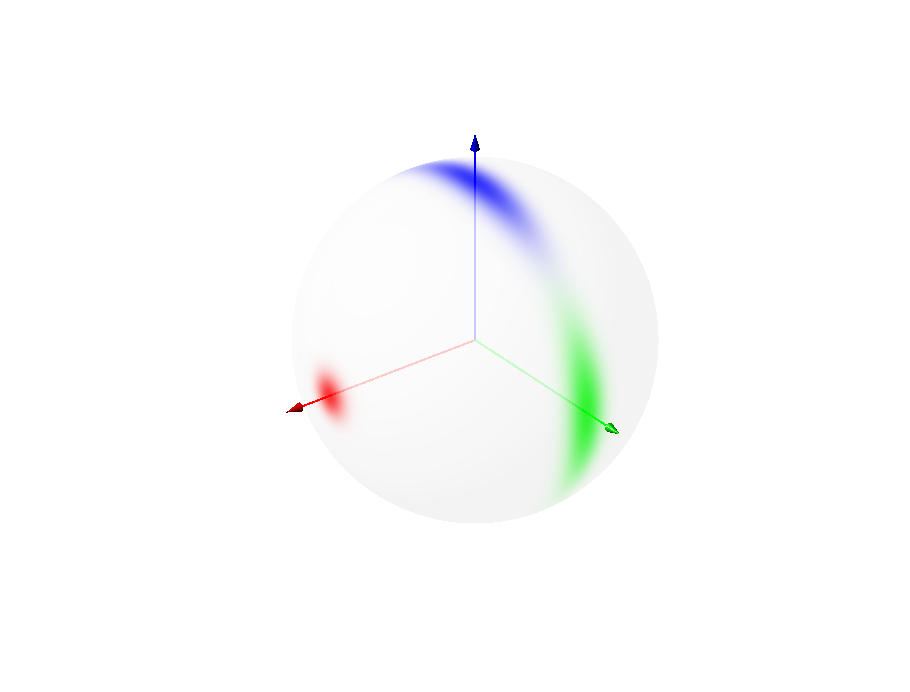
\includegraphics[width=0.2\columnwidth, trim=100 60 100 40, clip]{prop_L_1}};
				\node[opacity=1.0,outer sep=0pt,inner sep=0pt] at (0,0.1) {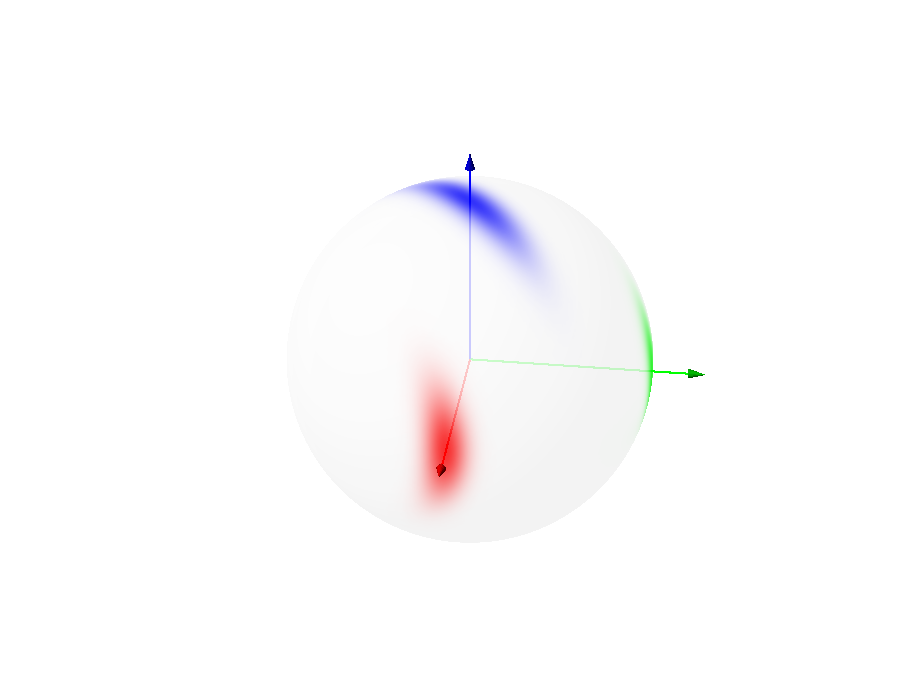
\includegraphics[width=0.2\columnwidth, trim=100 60 100 40, clip]{prop_L_2}};
				\node[opacity=1.0,outer sep=0pt,inner sep=0pt] at (3.0,0.1) {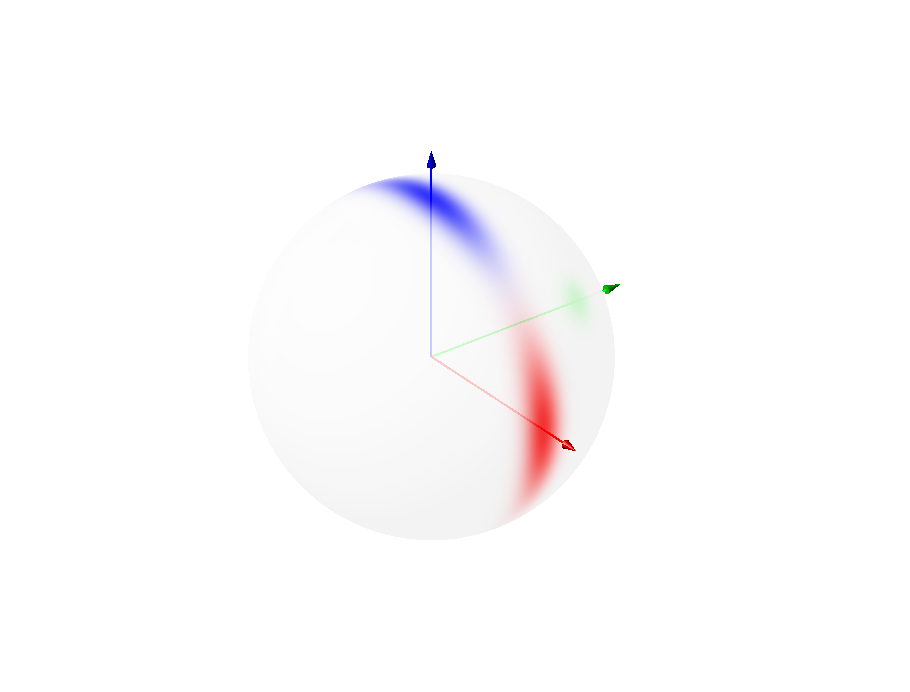
\includegraphics[width=0.2\columnwidth, trim=100 60 100 40, clip]{prop_L_3}};
				\node[opacity=1.0,outer sep=0pt,inner sep=0pt] at (-2.9,-1.1) {\scriptsize $t=0$s};
				\node[opacity=1.0,outer sep=0pt,inner sep=0pt] at (0.1,-1.1) {\scriptsize $t=0.5$s};
				\node[opacity=1.0,outer sep=0pt,inner sep=0pt] at (3.0,-1.1) {\scriptsize $t=1$s};
				
				\draw[arrows={-Triangle[angle=30:3pt]}] (-1.4,-0.6) -- ++(90:0.4);
				\draw[arrows={-Triangle[angle=30:3pt]}] (-1.4,-0.6) -- ++(-30:0.4);
				\draw[arrows={-Triangle[angle=30:3pt]}] (-1.4,-0.6) -- ++(210:0.4);
				\node at (-1.75,-0.95) {\tiny $\bm{e}_1$};
				\node at (-0.95,-0.95) {\tiny $\bm{e}_2$};
				\node at (-1.37,-0.12) {\tiny $\bm{e}_3$};
			\end{tikzpicture}
		}
		
		\vspace{0.3cm}
		\item Angular velocity in inertial frame:  $\tfrac{\diff{R}(t)}{\diff{t}} = \hat{\omega}(t)R(t)$
		\begin{itemize}
			\item The uncertainty is unchanged in the body-fixed frame, but is rotated in the inertial frame.
		\end{itemize}
		
		\centerline{
			\begin{tikzpicture}
				\node[opacity=1.0,outer sep=0pt,inner sep=0pt] at (-3.0,0) {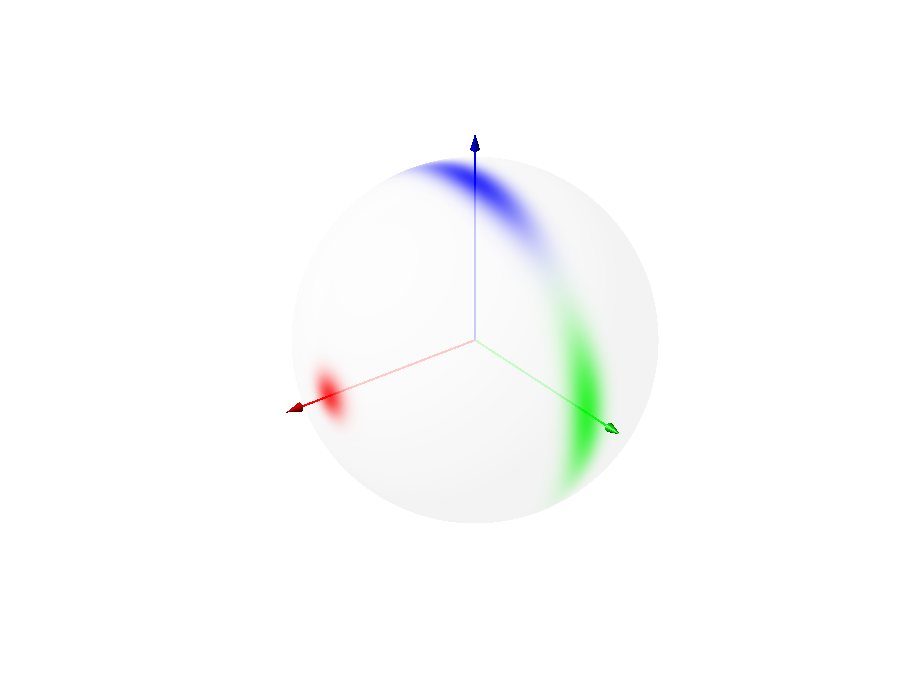
\includegraphics[width=0.2\columnwidth, trim=100 60 100 40, clip]{prop_R_1}};
				\node[opacity=1.0,outer sep=0pt,inner sep=0pt] at (0,0.1) {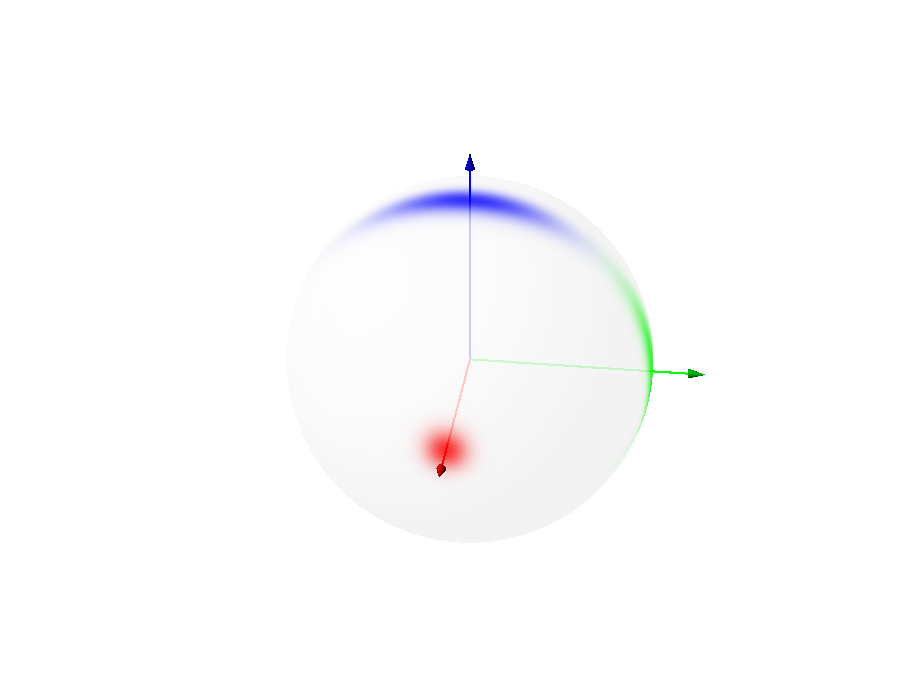
\includegraphics[width=0.2\columnwidth, trim=100 60 100 40, clip]{prop_R_2}};
				\node[opacity=1.0,outer sep=0pt,inner sep=0pt] at (3.0,0.1) {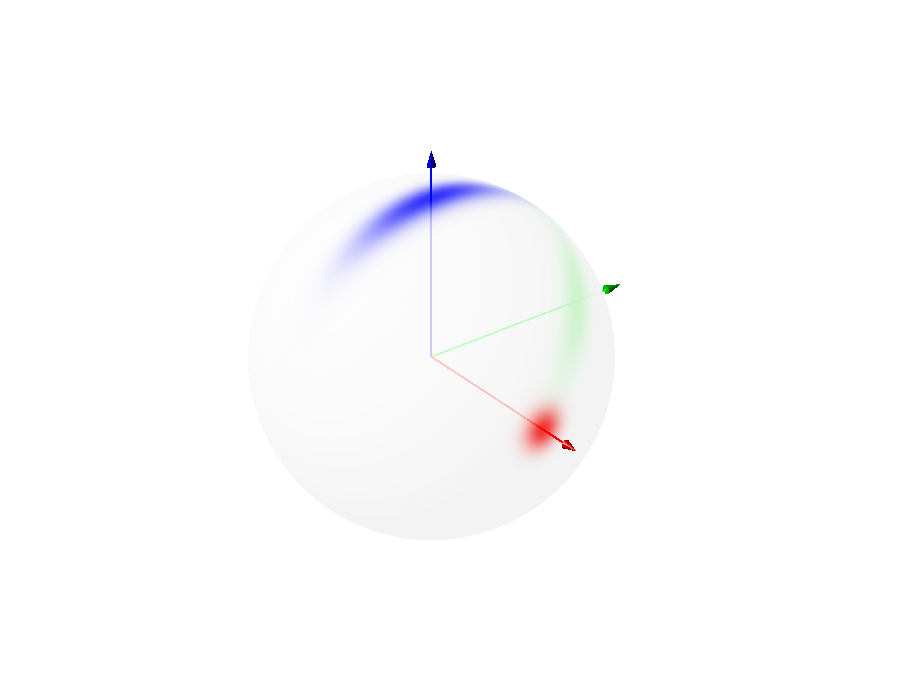
\includegraphics[width=0.2\columnwidth, trim=100 60 100 40, clip]{prop_R_3}};
				\node[opacity=1.0,outer sep=0pt,inner sep=0pt] at (-2.9,-1.1) {\scriptsize $t=0$s};
				\node[opacity=1.0,outer sep=0pt,inner sep=0pt] at (0.1,-1.1) {\scriptsize $t=0.5$s};
				\node[opacity=1.0,outer sep=0pt,inner sep=0pt] at (3.0,-1.1) {\scriptsize $t=1$s};
				
				\draw[arrows={-Triangle[angle=30:3pt]}] (-1.4,-0.6) -- ++(90:0.4);
				\draw[arrows={-Triangle[angle=30:3pt]}] (-1.4,-0.6) -- ++(-30:0.4);
				\draw[arrows={-Triangle[angle=30:3pt]}] (-1.4,-0.6) -- ++(210:0.4);
				\node at (-1.75,-0.95) {\tiny $\bm{e}_1$};
				\node at (-0.95,-0.95) {\tiny $\bm{e}_2$};
				\node at (-1.37,-0.12) {\tiny $\bm{e}_3$};
			\end{tikzpicture}
		}
	\end{itemize}
\end{frame}

\begin{frame}
	\frametitle{Correction From Direction Measurements}
	\begin{itemize}
		\item Reference direction in inertial frame: $x(t) = R(t)^Ta$
		\begin{itemize}
			\item Non-informative along direction $a$; $a$ is fixed in inertial frame.
		\end{itemize}
		
		\centerline{
			\begin{tikzpicture}
				\node[opacity=1.0,outer sep=0pt,inner sep=0pt] at (-3.0,0) {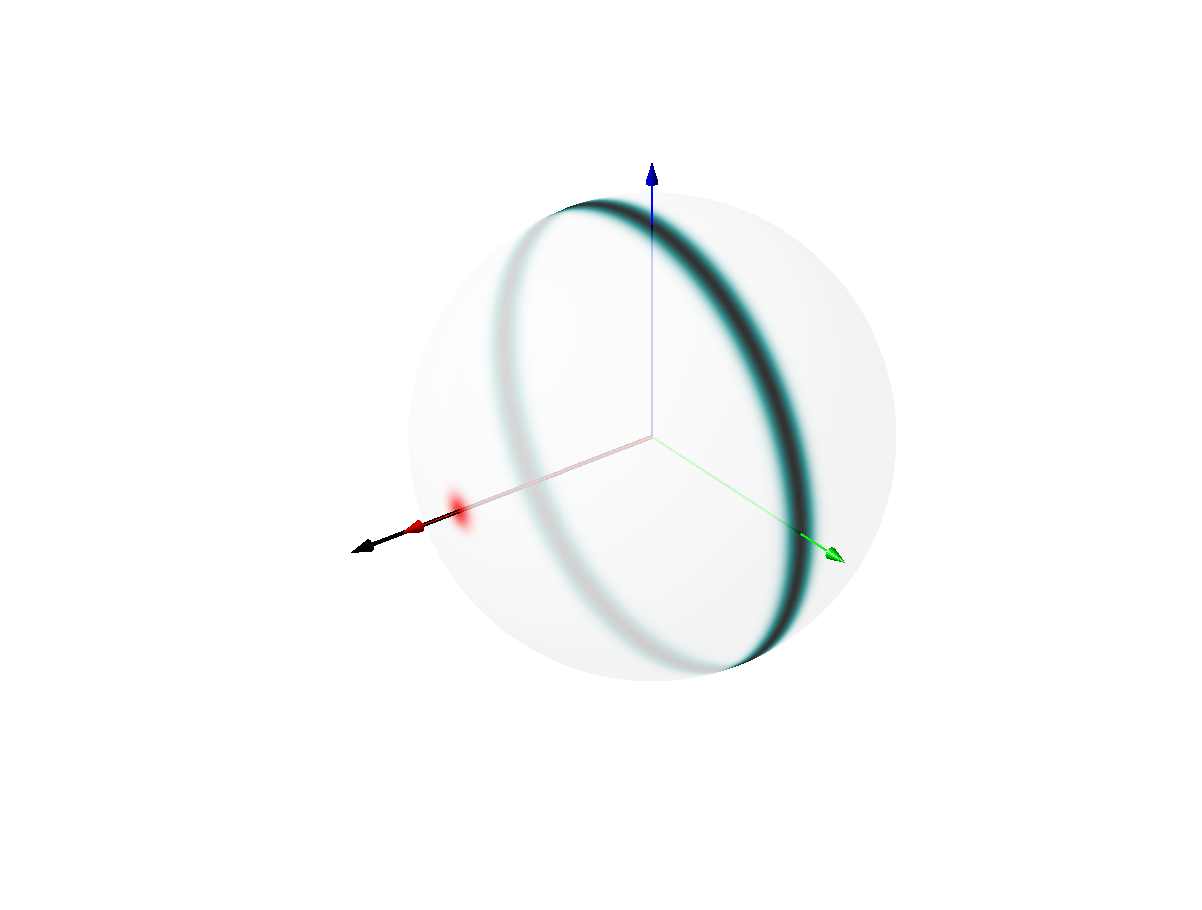
\includegraphics[width=0.2\columnwidth, trim=100 60 100 40, clip]{mea_I_1}};
				\node[opacity=1.0,outer sep=0pt,inner sep=0pt] at (0,0.1) {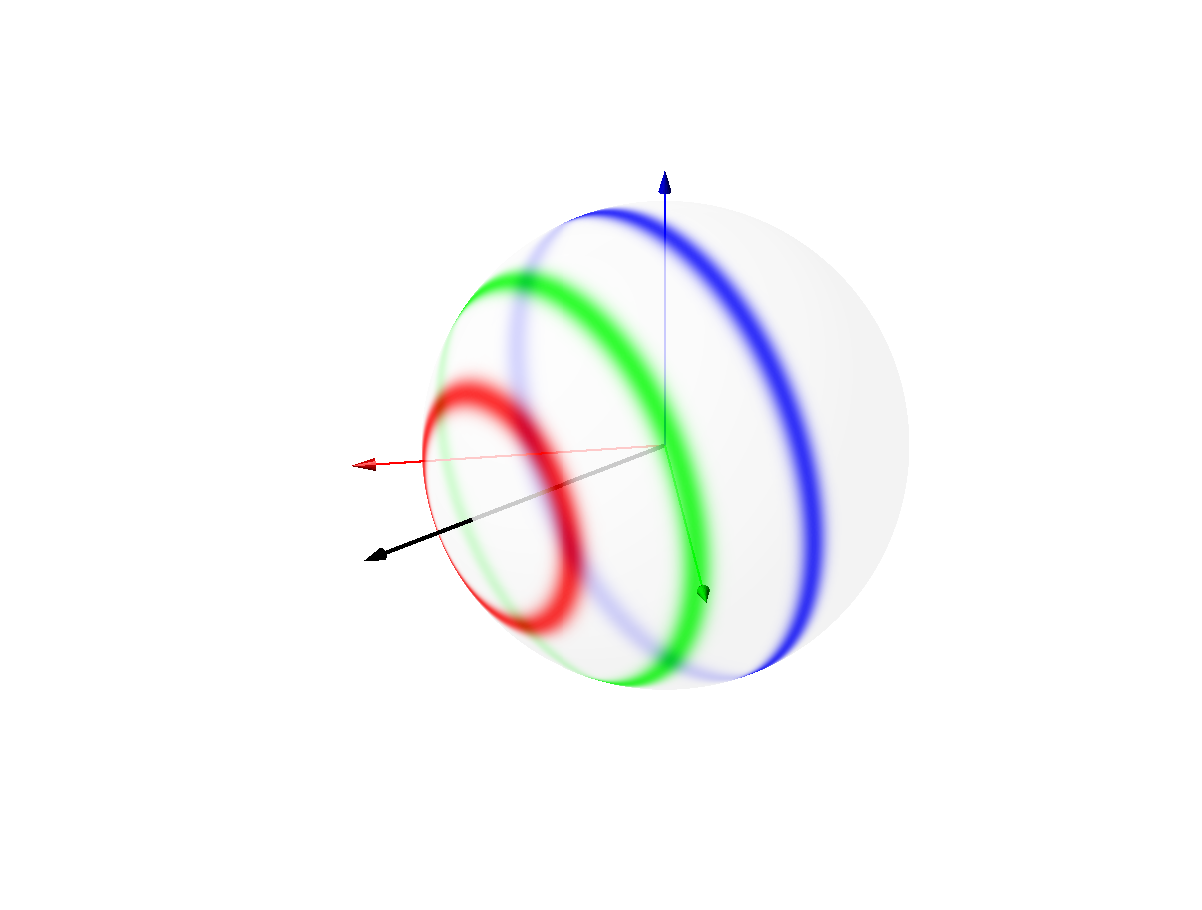
\includegraphics[width=0.2\columnwidth, trim=100 60 100 40, clip]{mea_I_2}};
				\node[opacity=1.0,outer sep=0pt,inner sep=0pt] at (3.0,0.1) {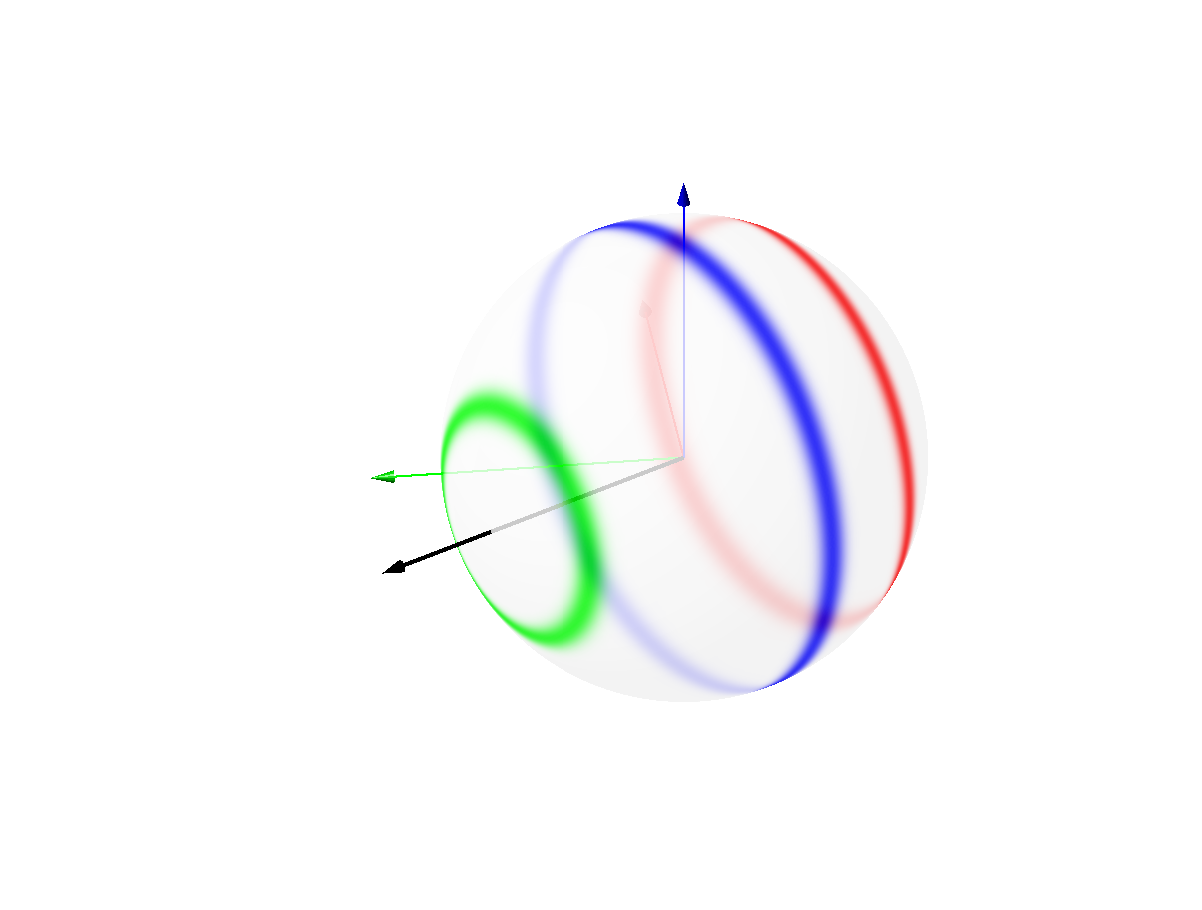
\includegraphics[width=0.2\columnwidth, trim=100 60 100 40, clip]{mea_I_3}};
				\node[opacity=1.0,outer sep=0pt,inner sep=0pt] at (-2.8,-1.1) {\scriptsize $x=e_1$};
				\node[opacity=1.0,outer sep=0pt,inner sep=0pt] at (0.2,-1.1) {\scriptsize $x=\tfrac{\sqrt{3}}{2}e_1 + \tfrac{1}{2}e_2$};
				\node[opacity=1.0,outer sep=0pt,inner sep=0pt] at (3.3,-1.1) {\scriptsize $x=-\tfrac{1}{2}e_1 + \tfrac{\sqrt{3}}{2}e_2$};
				
				\draw[arrows={-Triangle[angle=30:3pt]}] (-1.4,-0.6) -- ++(90:0.4);
				\draw[arrows={-Triangle[angle=30:3pt]}] (-1.4,-0.6) -- ++(-30:0.4);
				\draw[arrows={-Triangle[angle=30:3pt]}] (-1.4,-0.6) -- ++(210:0.4);
				\node at (-1.75,-0.95) {\tiny $\bm{e}_1$};
				\node at (-0.95,-0.95) {\tiny $\bm{e}_2$};
				\node at (-1.37,-0.12) {\tiny $\bm{e}_3$};
			\end{tikzpicture}
		}
		
		\vspace{0.3cm}
		\item Reference direction in body-fixed frame: $y(t) = R(t)b$
		\begin{itemize}
			\item Non-informative along direction $b$; $b$ is fixed in body-fixed frame.
		\end{itemize}
		
		\centerline{
			\begin{tikzpicture}
				\node[opacity=1.0,outer sep=0pt,inner sep=0pt] at (-3.0,0) {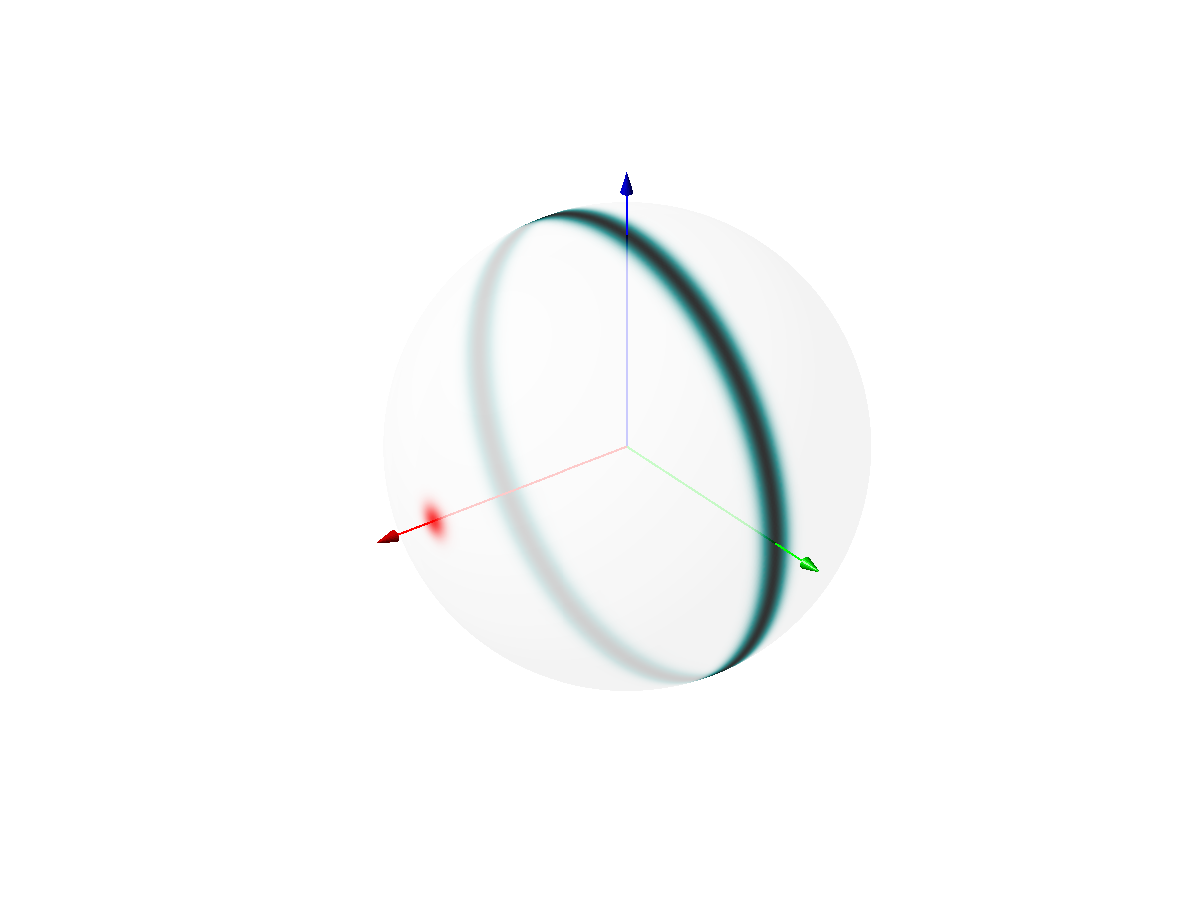
\includegraphics[width=0.2\columnwidth, trim=100 60 100 40, clip]{mea_B_1}};
				\node[opacity=1.0,outer sep=0pt,inner sep=0pt] at (0.0,0.1) {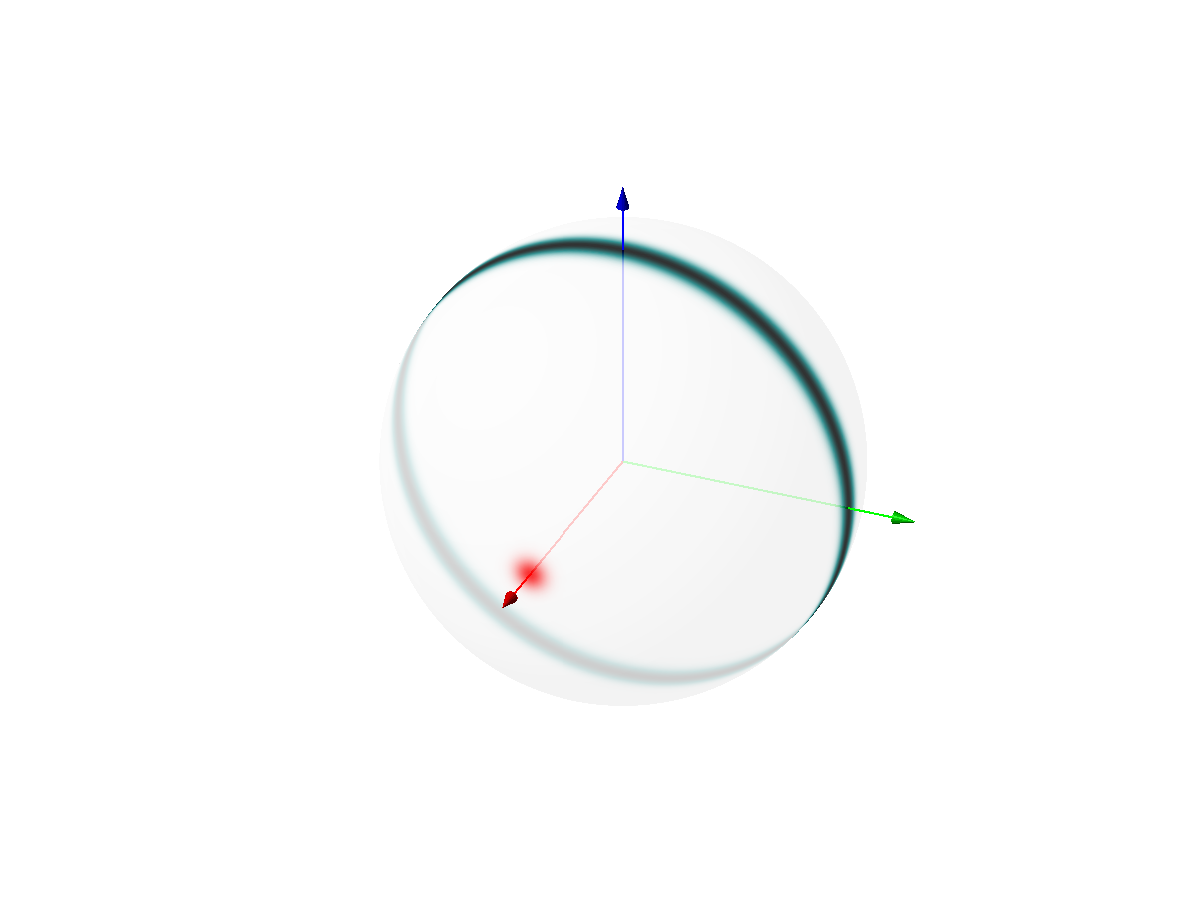
\includegraphics[width=0.2\columnwidth, trim=100 60 100 40, clip]{mea_B_2}};
				\node[opacity=1.0,outer sep=0pt,inner sep=0pt] at (3.0,0.1) {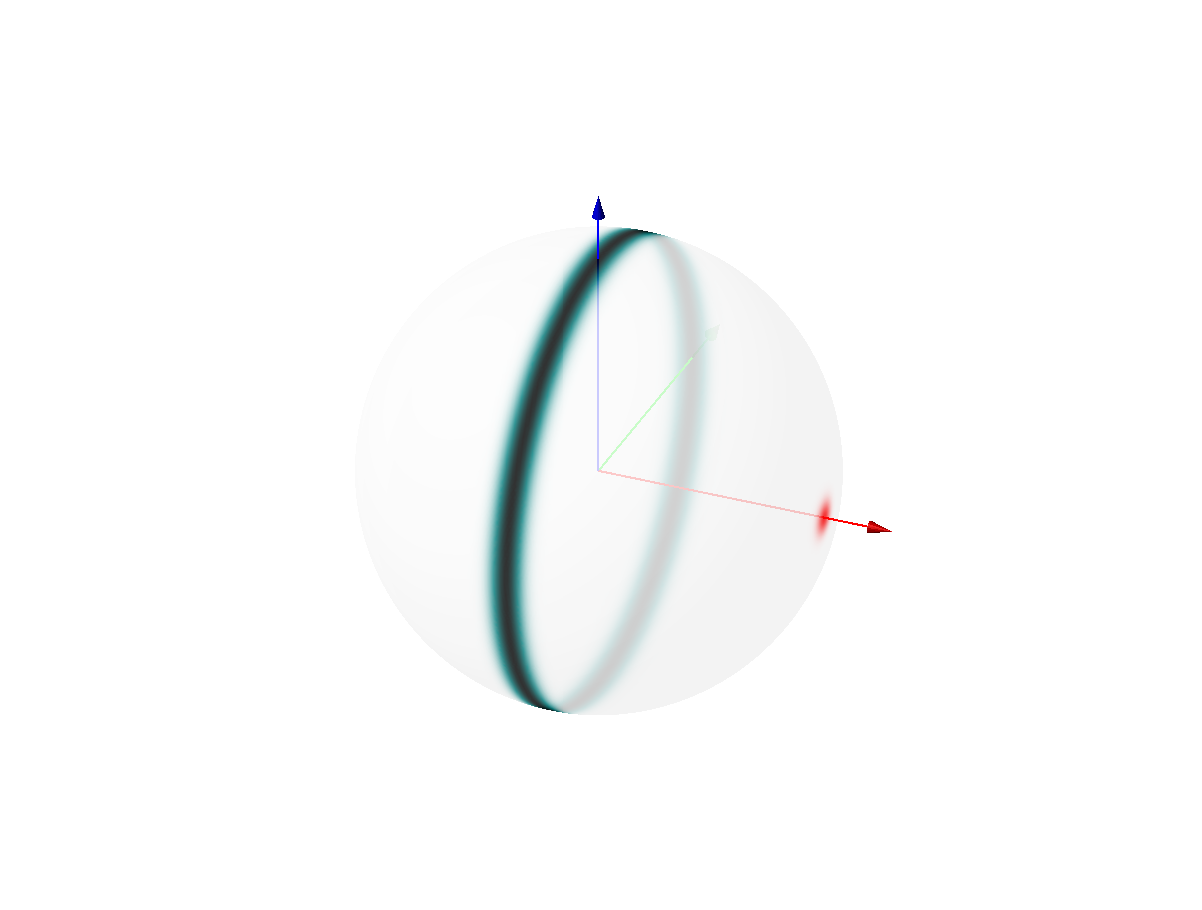
\includegraphics[width=0.2\columnwidth, trim=100 60 100 40, clip]{mea_B_3}};
				\node[opacity=1.0,outer sep=0pt,inner sep=0pt] at (-2.8,-1.1) {\scriptsize $y=e_1$};
				\node[opacity=1.0,outer sep=0pt,inner sep=0pt] at (0.2,-1.1) {\scriptsize $y=\tfrac{\sqrt{3}}{2}e_1 + \tfrac{1}{2}e_2$};
				\node[opacity=1.0,outer sep=0pt,inner sep=0pt] at (3.3,-1.1) {\scriptsize $y=-\tfrac{1}{2}e_1 + \tfrac{\sqrt{3}}{2}e_2$};
				
				\draw[arrows={-Triangle[angle=30:3pt]}] (-1.4,-0.6) -- ++(90:0.4);
				\draw[arrows={-Triangle[angle=30:3pt]}] (-1.4,-0.6) -- ++(-30:0.4);
				\draw[arrows={-Triangle[angle=30:3pt]}] (-1.4,-0.6) -- ++(210:0.4);
				\node at (-1.75,-0.95) {\tiny $\bm{e}_1$};
				\node at (-0.95,-0.95) {\tiny $\bm{e}_2$};
				\node at (-1.37,-0.12) {\tiny $\bm{e}_3$};
			\end{tikzpicture}
		}
	\end{itemize}
\end{frame}

\begin{frame}
	\frametitle{Observability}
	
	\begin{itemize}
		\item Observable:
		\begin{itemize}
			\item Angular velocity in body-fixed frame: $\tfrac{\diff{R}(t)}{\diff{t}} = R(t)\hat{\Omega}(t)$
			\item Reference direction in body-fixed frame: $y(t) = R(t)b$
		\end{itemize}
		
		\begin{figure}
			\centering
			\begin{tikzpicture}
				\node at (1.5,2.8) {\includegraphics[trim=150 80 120 60, clip, scale=0.23]{est_LB_F1_prior}};
				\node at (4.5,2.8) {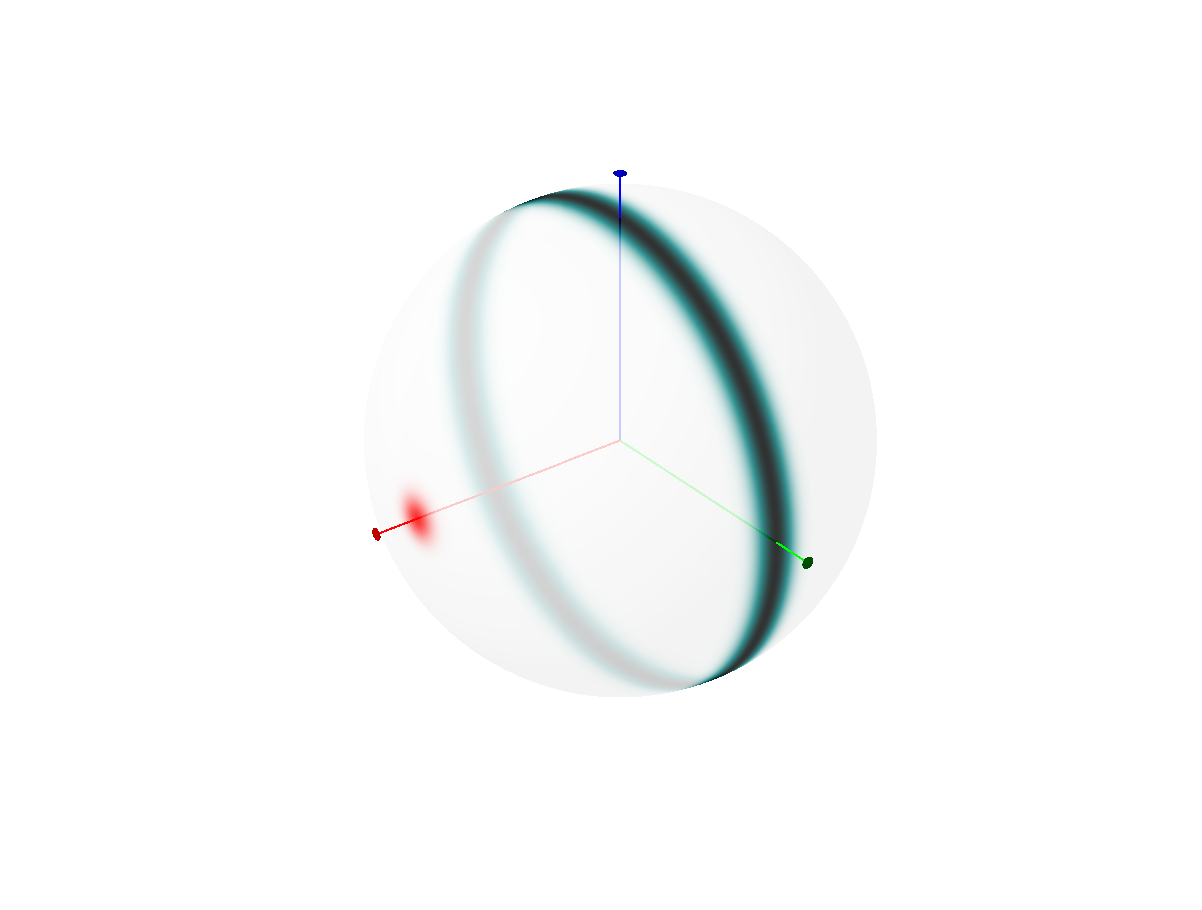
\includegraphics[trim=150 80 120 60, clip, scale=0.23]{est_LB_F1}};
				\node at (7.5,2.8) {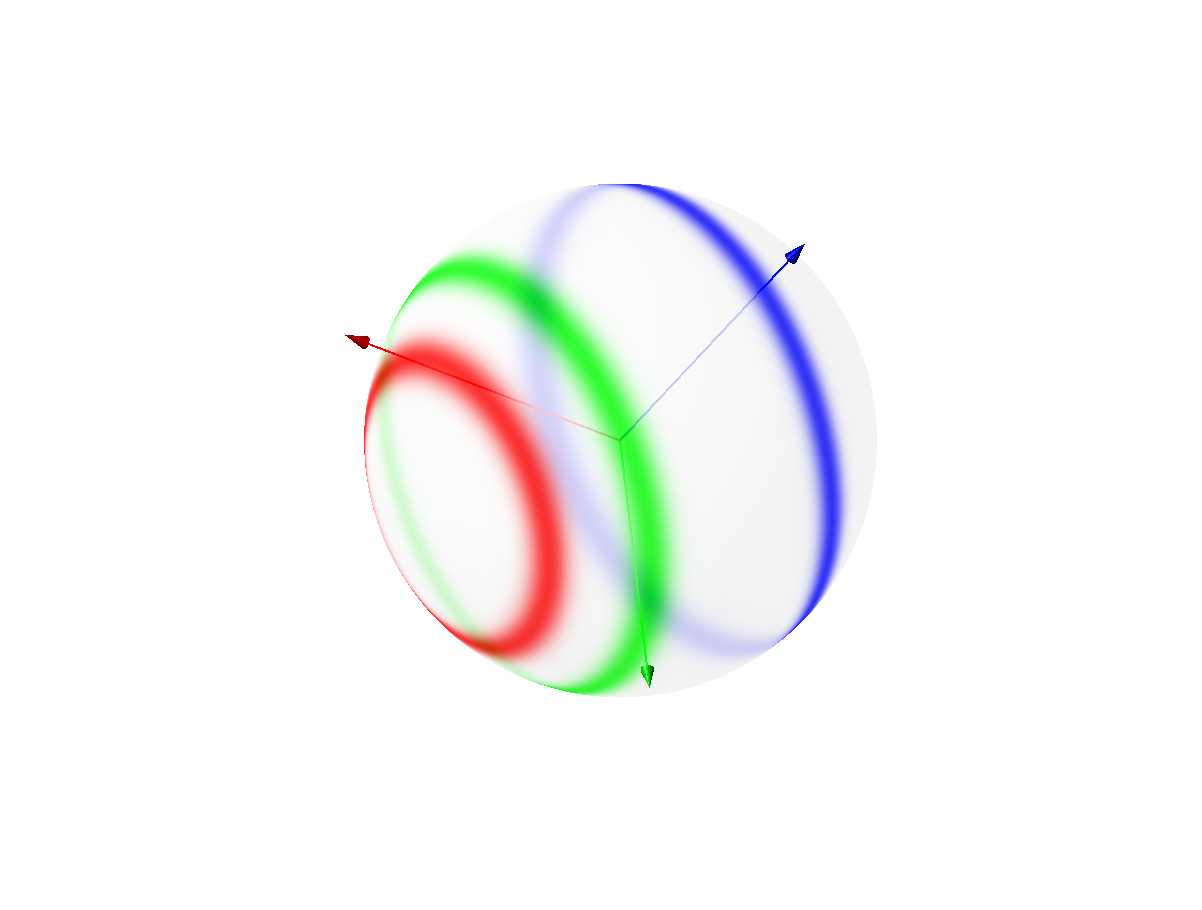
\includegraphics[trim=150 80 120 60, clip, scale=0.23]{est_LB_F3}};
				
				\node at (1.5,0) {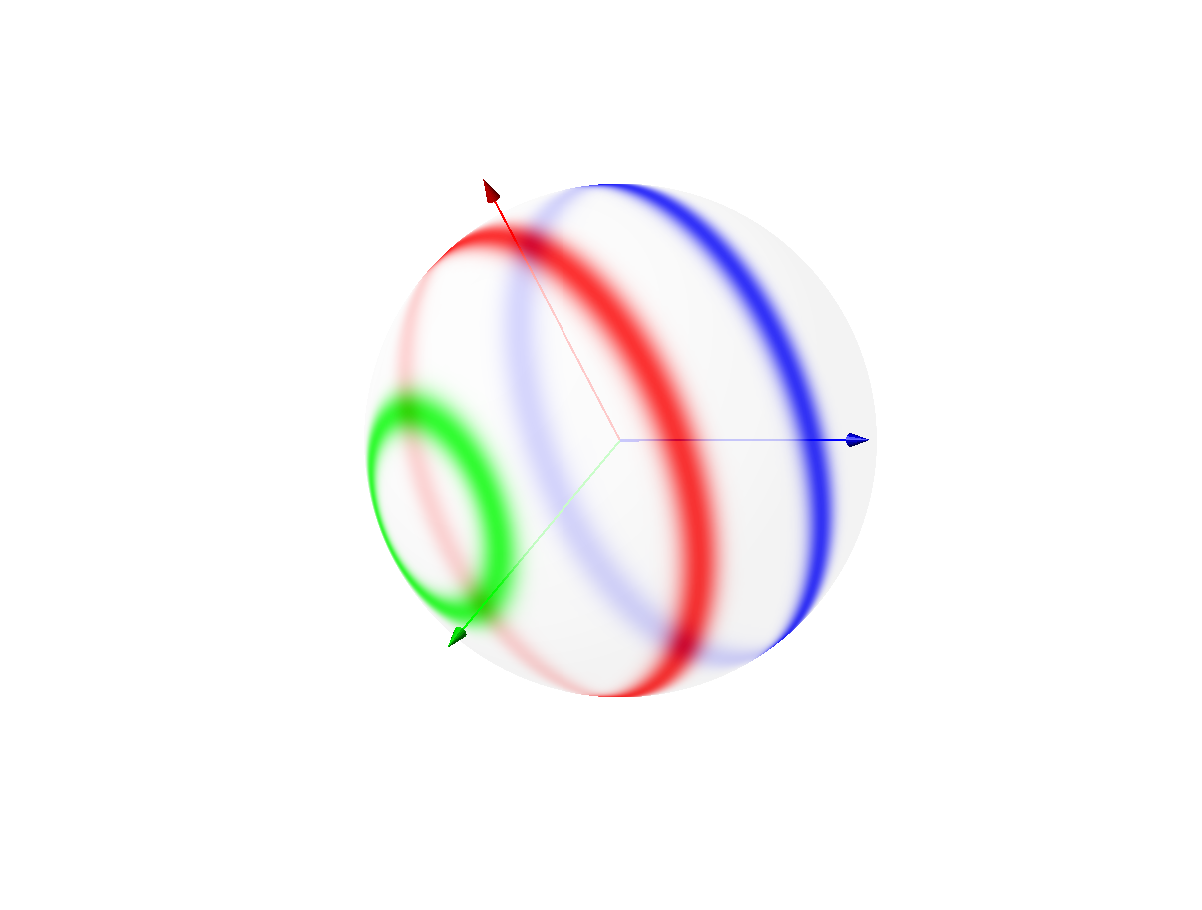
\includegraphics[trim=150 80 120 60, clip, scale=0.23]{est_LB_F5}};
				\node at (4.5,0) {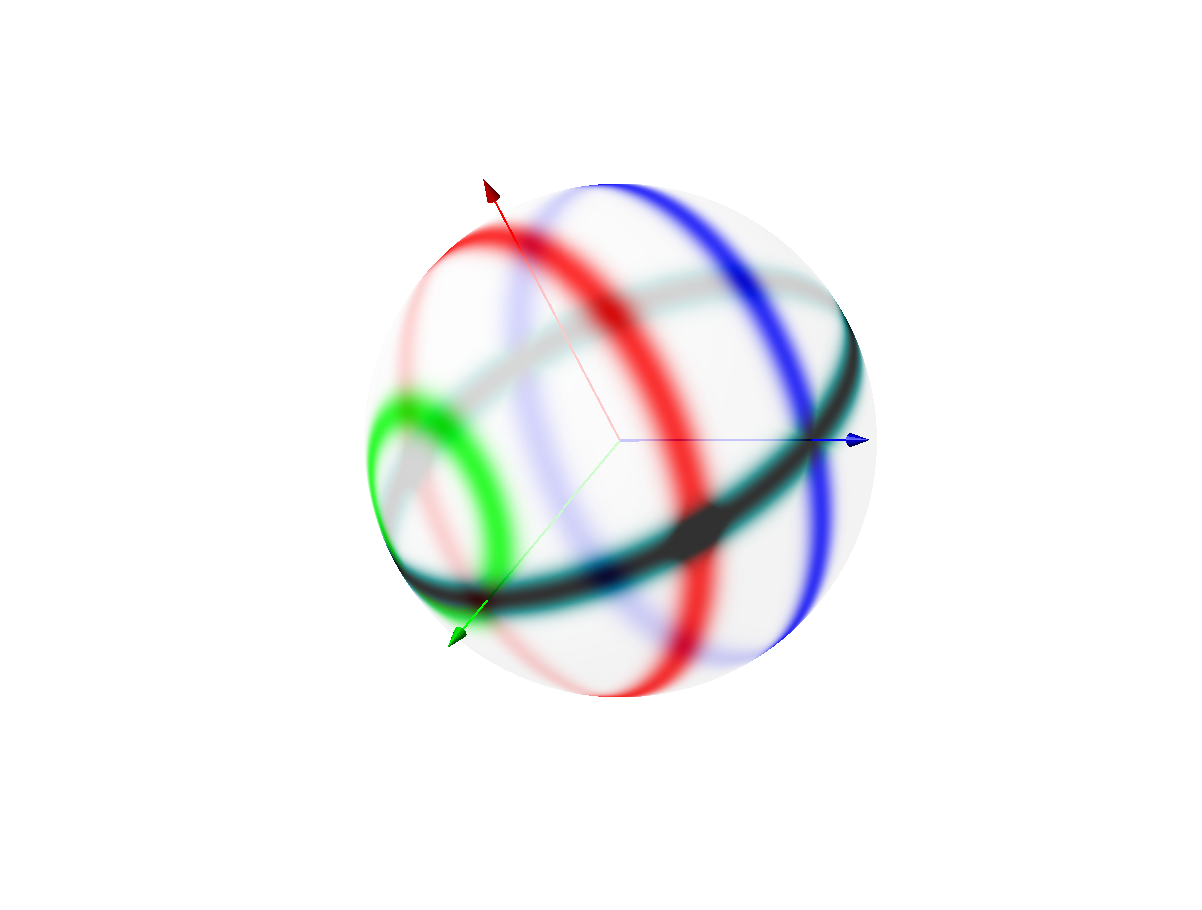
\includegraphics[trim=150 80 120 60, clip, scale=0.23]{est_LB_FN_mea}};
				\node at (7.5,0) {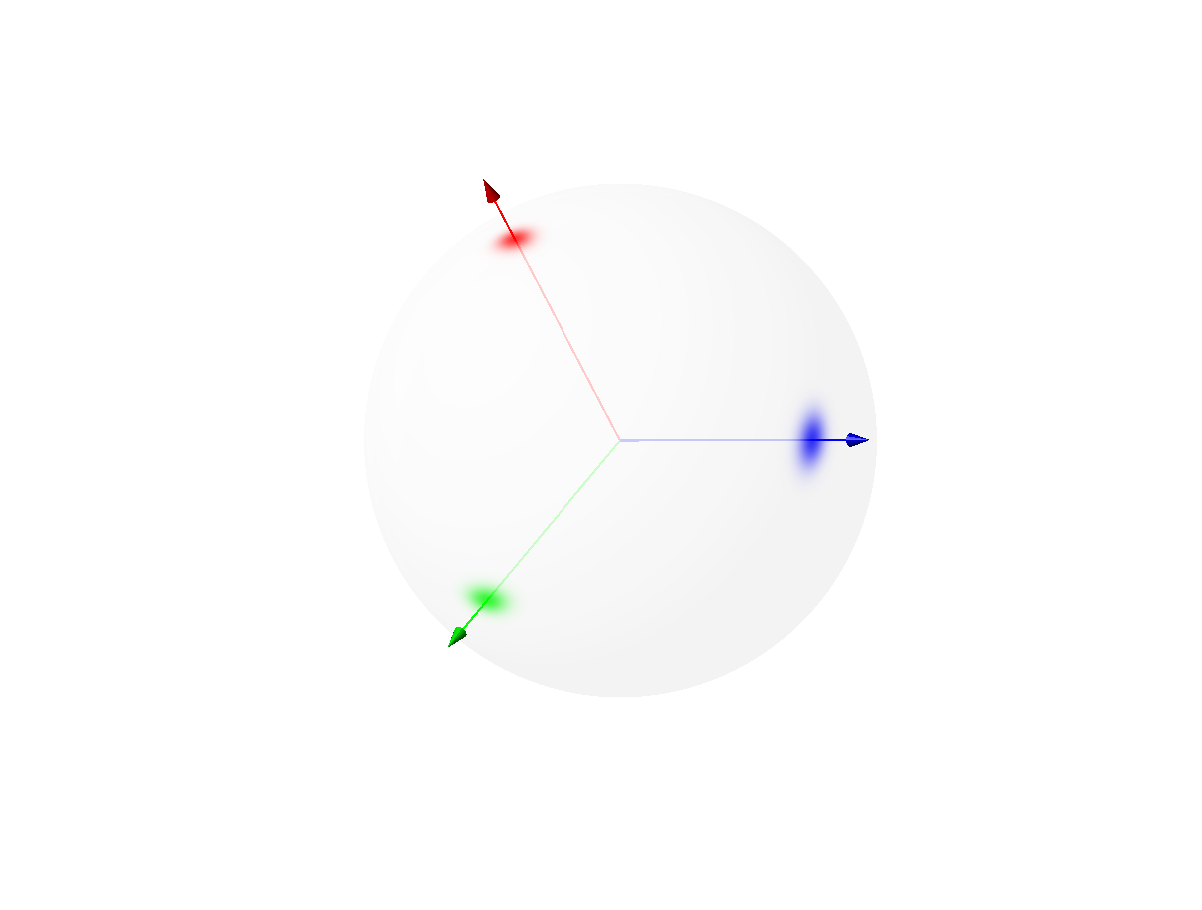
\includegraphics[trim=150 80 120 60, clip, scale=0.23]{est_LB_FN_post}};
				
				\draw[arrows={-Triangle[angle=30:3pt]}] (3.0,2.2) -- ++(90:0.4);
				\draw[arrows={-Triangle[angle=30:3pt]}] (3.0,2.2) -- ++(-30:0.4);
				\draw[arrows={-Triangle[angle=30:3pt]}] (3.0,2.2) -- 	++(210:0.4);
				\node at (2.65,1.85) {\tiny $\bm{e}_1$};
				\node at (3.45,1.85) {\tiny $\bm{e}_2$};
				\node at (3.03,2.68) {\tiny $\bm{e}_3$};
				
				\node at (1.5,1.5) {\scriptsize Prior dist. at $t=0$};
				\node at (4.4,1.5) {\scriptsize Posterior dist. at $t=0$};
				\node at (7.5,1.5) {\scriptsize Propagated dist. at $t=0.5$};
				
				\node at (1.5,-1.5) {\scriptsize Propagated dist. at $t=1$};
				\node[align=center] at (4.5,-1.5) {\parbox{0.28\textwidth}{\scriptsize Propagated dist. overlapped \\ with measured dist. at $t=1$}};
				\node at (7.5,-1.5) {\scriptsize Posterior dist. at $t=1$};
			\end{tikzpicture}
		\end{figure}
	\end{itemize}
\end{frame}

\begin{frame}
	\frametitle{Unobservability}
	
	\begin{itemize}
		\item Unobservable:
		\begin{itemize}
			\item Angular velocity in body-fixed frame: $\tfrac{\diff{R}(t)}{\diff{t}} = R(t)\hat{\Omega}(t)$
			\item Reference direction in inertial frame: $x(t) = R(t)^Ta$
		\end{itemize}
		
		\begin{figure}
			\centering
			\begin{tikzpicture}
				\node at (1.5,2.8) {
\includegraphics[trim=115 60 95 20, clip, scale=0.30]{est_LI_F1_prior}};
				\node at (4.5,2.8) {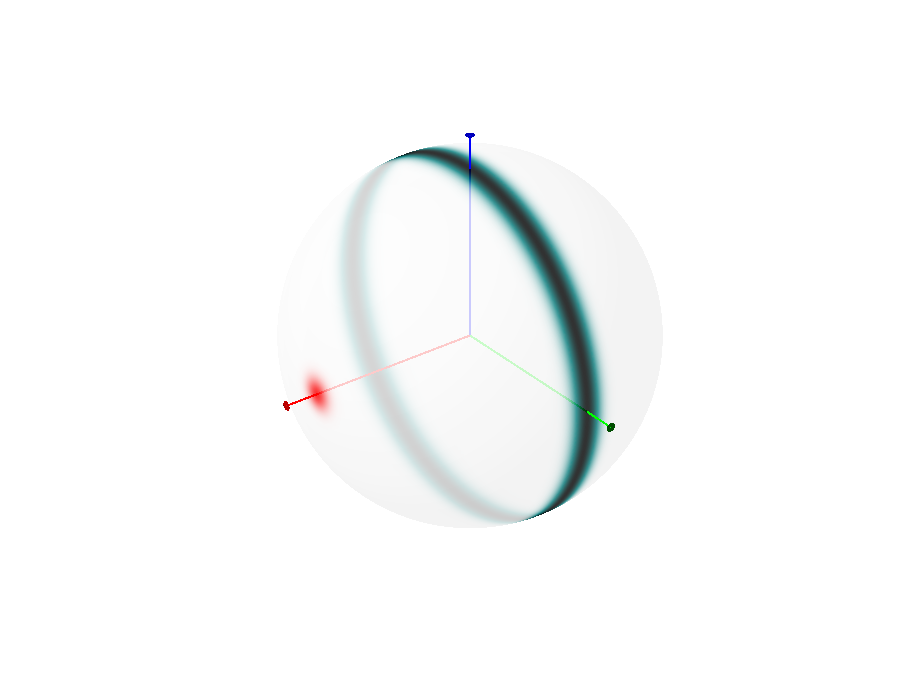
\includegraphics[trim=115 60 95 20, clip, scale=0.30]{est_LI_F1}};
				\node at (7.5,2.8) {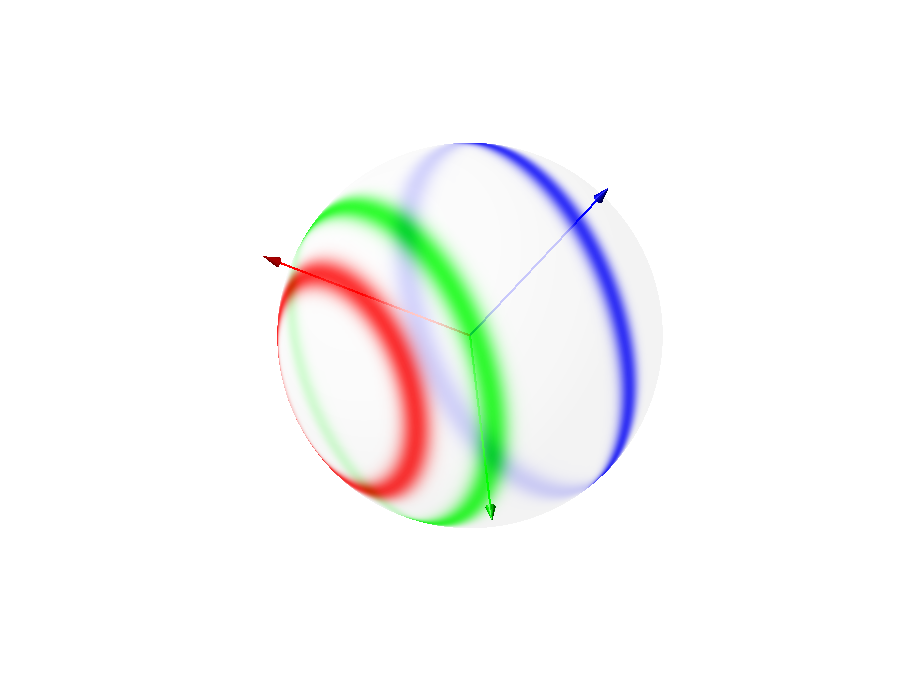
\includegraphics[trim=115 60 95 20, clip, scale=0.30]{est_LI_F3}};
				
				\node at (1.5,0) {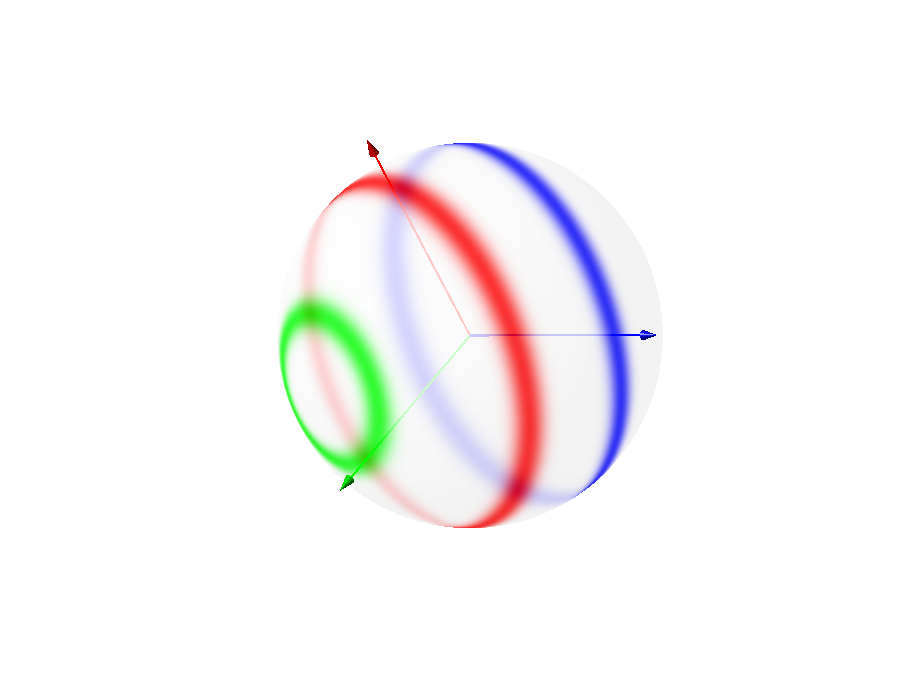
\includegraphics[trim=115 60 95 20, clip, scale=0.30]{est_LI_F5}};
				\node at (4.5,0) {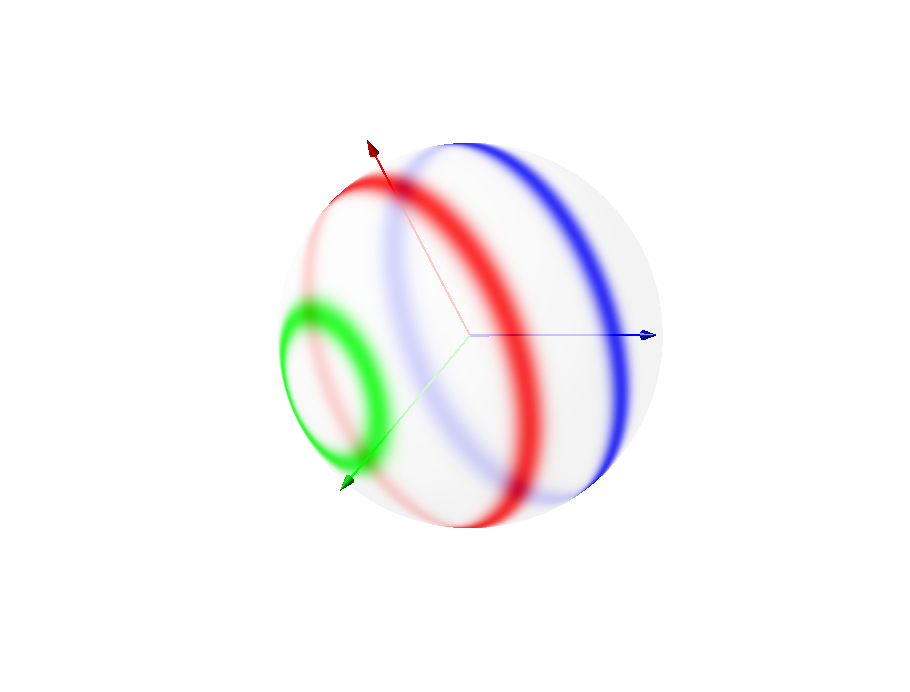
\includegraphics[trim=115 60 95 20, clip, scale=0.30]{est_LI_FN_mea}};
				\node at (7.5,0) {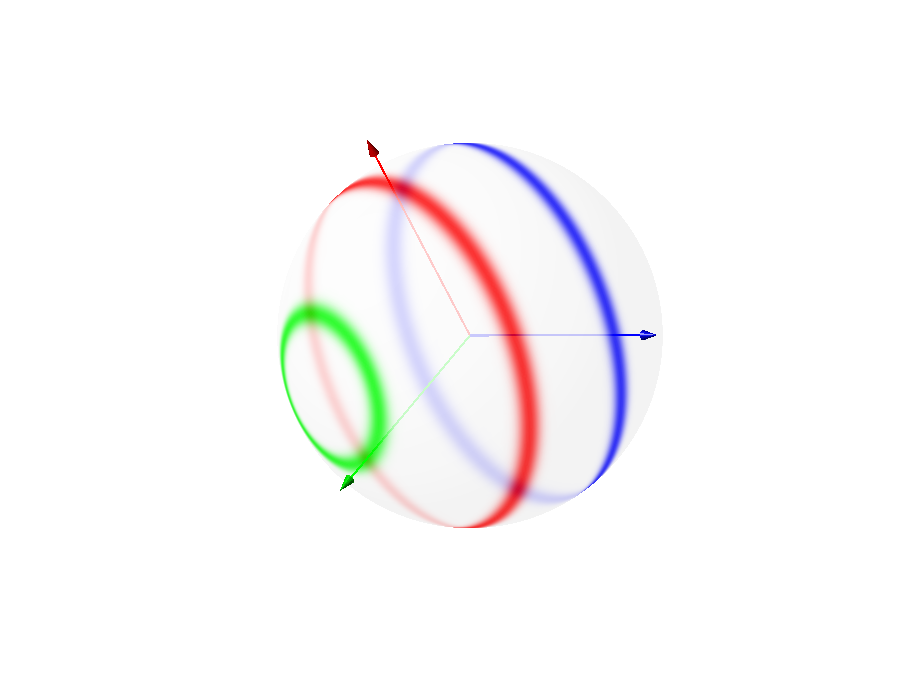
\includegraphics[trim=115 60 95 20, clip, scale=0.30]{est_LI_FN_post}};
				
				\draw[arrows={-Triangle[angle=30:3pt]}] (3.0,2.2) -- ++(90:0.4);
				\draw[arrows={-Triangle[angle=30:3pt]}] (3.0,2.2) -- ++(-30:0.4);
				\draw[arrows={-Triangle[angle=30:3pt]}] (3.0,2.2) -- 	++(210:0.4);
				\node at (2.65,1.85) {\tiny $\bm{e}_1$};
				\node at (3.45,1.85) {\tiny $\bm{e}_2$};
				\node at (3.03,2.68) {\tiny $\bm{e}_3$};
				
				\node at (1.5,1.4) {\scriptsize Prior dist. at $t=0$};
				\node at (4.4,1.4) {\scriptsize Posterior dist. at $t=0$};
				\node at (7.5,1.4) {\scriptsize Propagated dist. at $t=0.5$};
				
				\node at (1.5,-1.5) {\scriptsize Propagated dist. at $t=1$};
				\node[align=center] at (4.5,-1.5) {\parbox{0.28\textwidth}{\scriptsize Propagated dist. overlapped \\ with measured dist. at $t=1$}};
				\node at (7.5,-1.5) {\scriptsize Posterior dist. at $t=1$};
			\end{tikzpicture}
		\end{figure}
	\end{itemize}
\end{frame}

\begin{frame}
	\frametitle{Experimental Verification}
	
	\begin{center}
		\scriptsize
		\begin{tabular}{l|cc}
			\diagbox[width=10em]{ref. vec.}{ang. vel.} & \makecell{body-fixed frame \\ (1a)} & \makecell{inertial frame \\ (1b)} \\ \hline
			body-fixed frame (2a) & \color{red} AVB\_RVB & AVI\_RVB \\
			inertial frame (2b) & AVB\_RVI & \color{red} AVI\_RVI
		\end{tabular}
	\end{center}
	
	\only<1>{
		\begin{itemize}
			\item Attitude error \footnote{\scriptsize I would like to thank Kanishke Gamagedara for conducting the experiment.}
			
			\vspace{0.2cm}
			\begin{figure}
				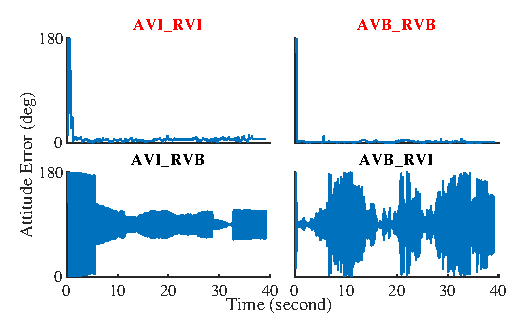
\includegraphics[scale=0.7]{attitudeError-Exp-MF}
			\end{figure}
			
			\begin{itemize}
				\item \color{red} AVB\_RVB \color{black} and \color{red} AVI\_RVI \color{black}: attitude error converges to around zero.
				\item AVB\_RVI and AVI\_RVB: attitude error does not converge.
			\end{itemize}
		\end{itemize}
	}
	
	\only<2>{
		\begin{itemize}
			\item Attitude uncertainty
			
			\vspace{0.2cm}
			\begin{figure}
				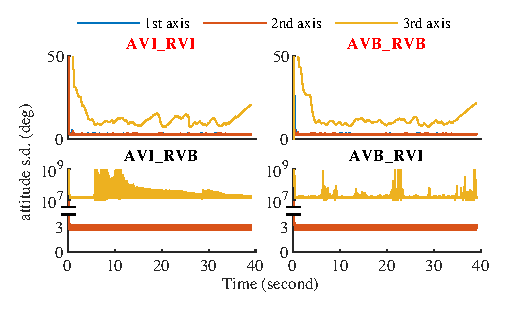
\includegraphics[scale=0.8]{attitudeStd-Exp-MF}
			\end{figure}
			
			\begin{itemize}
				\item \color{red} AVB\_RVB \color{black} and \color{red} AVI\_RVI \color{black}: standard deviations for all axes are small.
				\item AVB\_RVI and AVI\_RVB: standard deviation for one axis is large.
			\end{itemize}
		\end{itemize}
	}
\end{frame}

\subsection{Attitude Estimation Based on MFG}

\begin{frame}
	\frametitle{Attitude Estimation Based on MFG}
	\framesubtitle{Problem Formulation}
	
	\begin{itemize}
		\item Gyroscope Model
		
		\small
		\centerline{
			\begin{beamercolorbox}[wd=10cm,sep=0.0cm,center,rounded=true,shadow=true]{numerical}
				\vspace{-0.4cm}
				\begin{gather*}
					R_{k+1} = R_k \exp\left\{ h (\hat{\Omega}_k+\hat{x}_k) + (H_u\Delta W_u)^\wedge \right\}, \\
					x_{k+1} = x_k + H_v\Delta W_v.
				\end{gather*}
				\vspace{-0.6cm}
			\end{beamercolorbox}
		} \normalsize
		
		\begin{itemize}
			\item Angle random walk noise: $H_u\Delta W_u$.
			\item Bias random walk noise: $H_v\Delta W_v$.
		\end{itemize}
		
		\vspace{0.1cm}
		\item Measurement Model
		\begin{itemize}
			\item Attitude measurement: $Z_i = R_t\delta R$, $\delta R \sim \mathcal{M}(F_{Z_i})$, $i=1,\ldots,N_a$.
			\item Vector measurement: $z_j \in \mathbb{S}^2 \sim \mathcal{VM}(R^TB_ja_j,\kappa_j)$, $j = 1,\ldots,N_v$.
			\begin{itemize}
				\item $\mathcal{VM}$: von Mises--Fisher distribution on $\mathbb{S}^2$.
				\item $a_j$: a reference vector in the inertial frame.
			\end{itemize}
		\end{itemize}
		
		\vspace{0.1cm}
		\item Bayesian Assumed Density Filter
		\begin{itemize}
			\item Uncertainty propagation: $(R,x)_k^+ \sim \mathcal{MG}(\mu,\Sigma,P,U,S,V)_k^+$ $\Rightarrow (R,x)_{k+1}^- \sim \mathcal{MG}(\mu,\Sigma,P,U,S,V)_{k+1}^-$.
			\item Measurement update: $(R,x)_{k+1}^- \sim \mathcal{MG}(\mu,\Sigma,P,U,S,V)_{k+1}^-$ $\Rightarrow (R,x)_{k+1}^+ \sim \mathcal{MG}(\mu,\Sigma,P,U,S,V)_{k+1}^+$.
		\end{itemize}
	\end{itemize}
\end{frame}

\begin{frame}
	\frametitle{Uncertainty Propagation}
	
	\begin{itemize}
		\item Analytical Propagation
		\begin{itemize}
			\item Calculate analytical approximations $O(h^2)$ of moments for MLE.
			\item Marginal MLE: $\expect{R_{k+1}^-} \to U_{k+1}^-, S_{k+1}^-, V_{k+1}^-$.
			\item Conditional MLE: $\expect{x_{k+1}^-}$, $\expect{\nu_{R_{k+1}}^-}$, $\expect{xx^T}_{k+1}^-$, $\expect{x\nu_R^T}_{k+1}^-$, $\expect{\nu_R\nu_R^T}_{k+1}^- \Rightarrow \mu_{k+1}^-, \Sigma_{k+1}^-, P_{k+1}^-$.
		\end{itemize}
		
		\vspace{0.2cm}
		\item Unscented Propagation
		\begin{itemize}
			\item Select sigma points $(R_i,x_i,w_i)_{i=1}^{13}$ from $\mathcal{MG}(\mu,\Sigma,P,U,S,V)_k^+$.
			\item Select sigma points $(\eta_j,w_j)_{j=1}^7$ from noise $H_u\Delta W_u$.
			\item Propagate sigma points through the kinematic equations.
			
			\centerline{
				\begin{beamercolorbox}[wd=10cm,sep=0.0cm,center,rounded=true,shadow=true]{numerical}
					\vspace{-0.5cm}
					\begin{align*}
						R_{ij} = R_i\exp(h(\hat{\Omega}_k+\hat{x}_k) + \hat{\eta}_j), \qquad x_{ij} = x_i
					\end{align*}
					\vspace{-0.6cm}
				\end{beamercolorbox}
			}
			
			\item Update weights: $w_{ij} = w_iw_j$.
			\item Recover $\mathcal{MG}_{k+1}^-$ from the sigma points $(R_{ij},x_{ij},w_{ij})_{i=1,j=1}^{i=13,j=7}$ using MLE.
			\item Set $\Sigma_{k+1}^- = \Sigma_{k+1}^- + hH_vH_v^T$.
		\end{itemize}
	\end{itemize}
\end{frame}

\begin{frame}
	\frametitle{Measurement Update}
	
	\begin{itemize}
		\item Measurement Model
		\begin{itemize}
			\item Attitude measurement: $Z_i = R_t\delta R$, $\delta R \sim \mathcal{M}(F_{Z_i})$, $i=1,\ldots,N_a$.
			\item Vector measurement: $z_j \in \mathbb{S}^2 \sim \mathcal{VM}(R_j^TB_ja_j,\kappa_j)$, $j = 1,\ldots,N_v$.
		\end{itemize}
		
		\vspace*{0.2cm}
		\item Bayes's formula
		
		\small
		\centerline{
			\begin{beamercolorbox}[wd=10cm,sep=0.0cm,center,rounded=true,shadow=true]{numerical}
				\vspace{-0.4cm}
				\begin{align*}
					&p(x,R \;\lvert\; Z_{1:N_a}, z_{1:N_v}) \propto p(x,R) \cdot p(Z_{1:N_a}, z_{1:N_v} \;\lvert\; x,R) \\
					=\; &\mathrm{etr}\bigg\{ \Big( F+\sum_{i=1}^{N_a}Z_iF_i^T+\sum_{j=1}^{N_v}\kappa_jB_j{a}_j{z}_j^T \Big)R^T \bigg\} \cdot  \expb{-\tfrac{1}{2}(x-{\mu}_c)^T{\Sigma}_c^{-1}(x-{\mu}_c)}
				\end{align*}
				\vspace{-0.4cm}
			\end{beamercolorbox}
		}
		
		\normalsize
		\vspace*{0.2cm}
		\item Match to a New MFG
		\begin{itemize}
			\item Marginal MLE:
			\begin{itemize}
				\item $U_{k+1}^+S_{k+1}^+(V_{k+1}^+)^T = F+\sum_{i=1}^{N_a}Z_iF_i^T+\sum_{j=1}^{N_v}\kappa_jB_j{a}_j{z}_j^T$.
			\end{itemize}
		
			\item Conditional MLE: 
			\begin{itemize}
				\item Calculate $\expect{x_{k+1}^+}$, $\expect{xx^T}_{k+1}^+$, $\expect{x\nu_R^T}_{k+1}^+$, $\expect{\nu_R\nu_R^T}_{k+1}^+$.
				\item $\Rightarrow \mu_{k+1}^+$, $\Sigma_{k+1}^+$, $P_{k+1}^+$.
			\end{itemize}
		\end{itemize}
	\end{itemize}
\end{frame}

\begin{frame}
	\frametitle{Simulations with Two Direction Measurements}
	
	\begin{itemize}
		\item Settings
		\begin{itemize}
			\item False initial conditions.
			\item Two direction measurements: accurate and inaccurate.
			\begin{itemize}
				\item Uncertainty around the first reference direction is very large.
				\item Uncertainties in the two other axes are small.
			\end{itemize}
		\end{itemize}
		
		\vspace{0.15cm}
		\item Estimation Errors
		\begin{itemize}
			\item Compared with MEKF: the state of art method. 
			\item MFG has \Emph{better accuracy} around the first reference direction.
			\item MFG has \Emph{faster convergence} with false initial values.
		\end{itemize}
		
		\vspace{0.15cm}	
		\centerline{
			\begin{tikzpicture}
				\node[opacity=1.0,outer sep=0pt,inner sep=0pt] at (0,0) {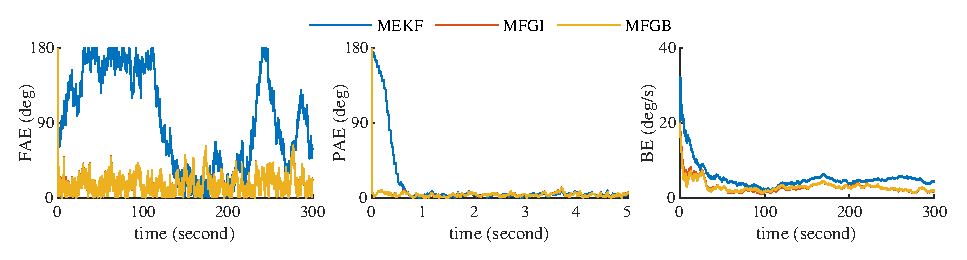
\includegraphics[scale=0.65]{attVec}};
			\end{tikzpicture}
		}
	\end{itemize}
\end{frame}

\begin{frame}
	\frametitle{Simulations with Single Direction Measurements}
	
	\begin{itemize}
		\item Settings
		\begin{itemize}
			\item A spacecraft orbiting around the Earth.
			\item False initial conditions.
			\item Time-varying magnetic field direction measurements.
			\begin{itemize}
				\item Uncertainty around the magnetic field is very large.
				\item Uncertainties in the two other axes are small.
			\end{itemize}
		\end{itemize}
		
		\vspace{0.15cm}
		\item Estimation Errors
		\begin{itemize}
			\item MFG has \Emph{better accuracy} around the magnetic field.
			\item MFG has \Emph{better accuracy} of gyroscope bias.
			\item MFGB is more accurate than MFGI.
		\end{itemize}
		
		\vspace{0.15cm}
		\centerline{
			\begin{tikzpicture}
				\node[opacity=1.0,outer sep=0pt,inner sep=0pt] at (0,0) {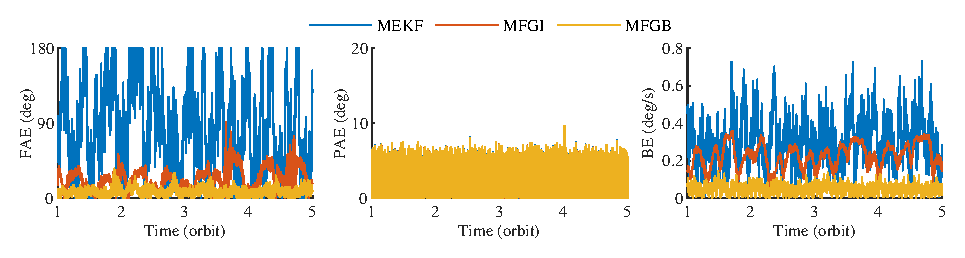
\includegraphics[scale=0.65]{attMag}};
			\end{tikzpicture}
		}
	\end{itemize}
\end{frame}

\section{6D Pose Estimation With MFG}

\begin{frame}
	\begin{itemize}
		\item Loosely Coupled IMU-GNSS Integration
		\item Visual-Inertial Navigation
	\end{itemize}
\end{frame}

\subsection{Loosely Coupled IMU-GNSS Integration}

\begin{frame}
	\frametitle{Loosely Coupled IMU-GNSS Integration}
	\framesubtitle{Problem Formulation}
	
	\begin{itemize}
		\item IMU Kinematics
		
		\centerline{
			\begin{beamercolorbox}[wd=10cm,sep=0.0cm,center,rounded=true,shadow=true]{numerical}
				\small
				\vspace{-0.3cm}
				\begin{align*}
					R_{k+1} &= R_k \expb{ h(\hat{\Omega}_k + \hat{b}_{g,k}) + H_{gu}\Delta W_{gu} }, \\
					b_{g,k+1} &= b_{g,k} + H_{gv}\Delta W_{gv}, \\
					p_{k+1} &= p_k + hv_k, \\
					v_{k+1} &= v_k - gh + R_k\left( h(a_k+b_{a,k}) + H_{au}\Delta W_{au} \right), \\
					b_{a,k+1} &= b_{a,k} + H_{av}\Delta W_{av}.
				\end{align*}
				\vspace{-0.4cm}
			\end{beamercolorbox}
		}
	
		\begin{itemize}
			\item $x = [b_g,p,v,b_a]\in\mathbb{R}^{12}$, where $b_g, b_a$ are gyroscope and accelerometer biases, and $v,p$ are velocity and position.
		\end{itemize}
	
		\vspace{0.2cm}
		\item Measurements
		\begin{itemize}
			\item Attitude and direction measurements (optional).
			\item GNSS receiver: position measurements.
			
			\centerline{
				\begin{beamercolorbox}[wd=10cm,sep=0.0cm,center,rounded=true,shadow=true]{numerical}
					\small
					\vspace{-0.3cm}
					\begin{align*}
						y_k|p_k = p_k + \mathcal{N}(0,\Sigma_y).
					\end{align*}
					\vspace{-0.4cm}
				\end{beamercolorbox}
			}
		\end{itemize}
	\end{itemize}
\end{frame}

\begin{frame}
	\frametitle{Bayesian Assumed Density Filter}
	
	\begin{itemize}
		\item Uncertainty Propagation
		\begin{itemize}
			\item Calculate analytical approximations $O(h^2)$ of moments.
			\item Use MLE to match the propagated moments to an MFG.
		\end{itemize}
		
		\vspace{0.2cm}
		\item Measurement Update
		\begin{itemize}
			\item Posterior probability density
			
			\centerline{
				\begin{beamercolorbox}[wd=10cm,sep=0.0cm,center,rounded=true,shadow=true]{numerical}
					\footnotesize
					\vspace{-0.3cm}
					\begin{align*}
						&p(R,x\lvert \mathcal{Z}) \propto \mathrm{etr} \bigg\{ \Big( F + \sum_{i=1}^{N_a}Z_iF_i^T + \sum_{j=1}^{N_v}\kappa_jB_ja_jz_j^T \Big)R^T \bigg\} \nonumber \\
						&\quad \cdot \expb{-\tfrac{1}{2}(x-\mu_c)^T\Sigma_c^{-1}(x-\mu_c)} \cdot \expb{-\tfrac{1}{2}(Hx-y)^T\Sigma_y^{-1}(Hx-y)}.
					\end{align*}
					\vspace{-0.4cm}
				\end{beamercolorbox}
			}
		
			\item Factorization of posterior probability density
			
			\centerline{
				\begin{beamercolorbox}[wd=10cm,sep=0.0cm,center,rounded=true,shadow=true]{numerical}
					\footnotesize
					\vspace{-0.3cm}
					\begin{align*}
						p(R,x|\mathcal{Z}) &\propto \Emph{p_R(R)} \cdot \Emph{p_{x|R}(x|R)}, \\
						\Emph{p_R(R)} &= \etr{\tilde{F}R^T} \expb{-\tfrac{1}{2}(H\mu_c-y)^T (\Sigma_y+H\Sigma_cH^T)^{-1} (H\mu_c-y)}, \\
						\Emph{p_{x|R}(x|R)} &= \expb{-\tfrac{1}{2} \big(x-K_p\mu_c-K_my\big)^T \big((I-K_mH)\Sigma_c\big)^{-1} \big(x-K_p\mu_c-K_my\big)}.
					\end{align*}
					\vspace{-0.4cm}
				\end{beamercolorbox}
			}
			
			\item \Emph{Marginal likelihood for $p_R(R)$, conditional likelihood for $p_{x|R}(x|R)$}.
		\end{itemize}
	\end{itemize}
\end{frame}

\begin{frame}
	\frametitle{Progressive Unscented Measurement Update}
	
	\begin{itemize}
		\item Marginal Likelihood for \Emph{$p_R(R)$}.
		
		\centerline{
			\begin{beamercolorbox}[wd=10cm,sep=0.0cm,center,rounded=true,shadow=true]{numerical}
				\footnotesize
				\vspace{-0.3cm}
				\begin{align*}
					p_R(R) = \etr{\tilde{F}R^T} \expb{-\tfrac{1}{2}(H\mu_c-y)^T (\Sigma_y+H\Sigma_cH^T)^{-1} (H\mu_c-y)}.
				\end{align*}
				\vspace{-0.4cm}
			\end{beamercolorbox}
		}
	
		\begin{itemize}
			\item Unscented update
			\begin{itemize}
				\item Select sigma points $\{R_i,w_i\}_{i=1}^7$ from $\mathcal{M}(\tilde{F})$.
				\item Reweigh the weights by $w_i^+ = w_i f_m(R_i)$, where $f_m(R)$ is the second term on the right hand side.
				\item Calculate $\expect{R}^+$: $w_i^+ = w_i^+/\sum_{j=1}^7 w_j^+$, $\expect{R}^+ = \sum_{i=1} w_i^+ R_i$.
				\item Use the marginal MLE: $U^+D^+(V^+)^T = \expect{R}^+$, $d_i^+ = \frac{1}{c(S^+)} \frac{\partial c(S^+)}{\partial s_i^+}$.
				\item \Emph{Sample degeneration}: $w_i^+$ can be close to zero.
			\end{itemize}
		
			\item Progressive unscented update \footnote{\tiny U.~D. Hanebeck, ``{PGF} 42: Progressive {G}aussian filtering with a twist,'' in
				\emph{International Conference on Information Fusion}, 2013, pp. 1103--1110.}
			
			\centerline{
				\begin{beamercolorbox}[wd=10cm,sep=0.0cm,center,rounded=true,shadow=true]{numerical}
					\footnotesize
					\vspace{-0.3cm}
					\begin{align*}
						f_m(R) = f_m(R)^{\lambda_1} f_m(R)^{\lambda_2} \cdots f_m(R)^{\lambda_l}
					\end{align*}
					\vspace{-0.4cm}
				\end{beamercolorbox}
			}
		
			\begin{itemize}
				\item Update the weights progressively: $w_i^k = w_i f_m(R_i)^{\lambda_k}$.
				\item Avoid sample degeneration: $\frac{\min_i\{w_i^k\}}{\max_i\{w_i^k\}} < \tau$, where $0 < \tau < 1$.
			\end{itemize}
		\end{itemize}
	\end{itemize}
\end{frame}

\begin{frame}
	\frametitle{Conditional MLE}
	
	\centerline{
		\begin{beamercolorbox}[wd=10cm,sep=0.0cm,center,rounded=true,shadow=true]{numerical}
			\footnotesize
			\vspace{-0.3cm}
			\begin{align*}
				p(R,x|\mathcal{Z}) &\propto \etr{F^+R^T} \cdot \Emph{p_{x|R}(x|R)}, \\
				\Emph{p_{x|R}(x|R)} &= \expb{-\tfrac{1}{2} \big(x-K_p\mu_c-K_my\big)^T \big((I-K_mH)\Sigma_c\big)^{-1} \big(x-K_p\mu_c-K_my\big)}.
			\end{align*}
			\vspace{-0.4cm}
		\end{beamercolorbox}
	}

	\begin{itemize}
		\item Conditional MLE for \Emph{$p_{x|R}(x|R)$}.
		\begin{itemize}
			\item Calculate the moments $\expect{x}$, $\expect{xx^T}$, $\expect{x\nu_R^T}$, $\expect{\nu_R}$, $\expect{\nu_R\nu_R^T}$, with respect to the above density function.
			\item $\Rightarrow \mu^+$, $\Sigma^+$, $P^+$.
		\end{itemize}
	\end{itemize}
\end{frame}

\begin{frame}
	\frametitle{Simulations}
	
	\begin{itemize}
		\item Initial conditions: highly accurate pitch and roll, \Emph{reversed yaw}.
		\begin{itemize}
			\item For example from indoors to outdoors.
		\end{itemize}
		
		\vspace{0.2cm}
		\item Estimation Errors
		\begin{itemize}
			\item MFG has \Emph{Faster convergence} of yaw.
			\item MFG has \Emph{Better accuracy} of position and velocity.
		\end{itemize}
		
		\vspace{0.4cm}
		\centerline{
			\begin{tikzpicture}
				\node[opacity=1.0,outer sep=0pt,inner sep=0pt] at (0,0) {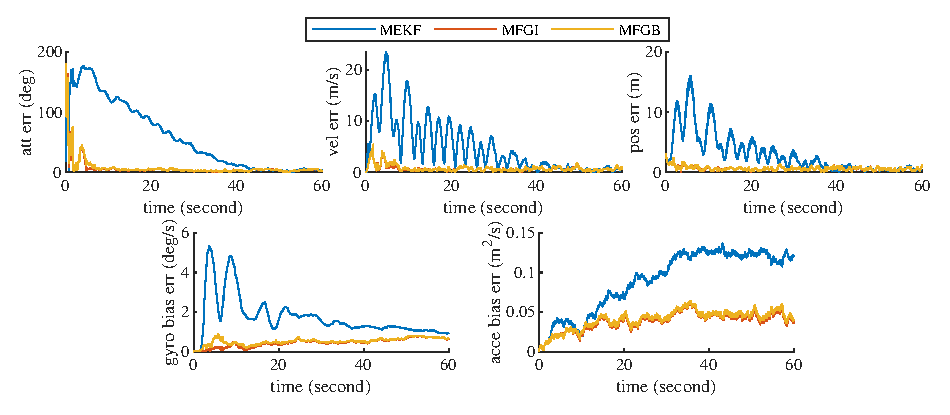
\includegraphics[scale=0.65]{INS_error}};
			\end{tikzpicture}
		}
	\end{itemize}
\end{frame}

\subsection{Visual-Inertial Navigation}

\begin{frame}
	\frametitle{Visual-Inertial Navigation}
	
	\begin{itemize}
		\item 3D Feature Location Measurements
		\begin{itemize}
			\item Camera types: RGB-D camera, stereo camera.
			\item Measures the coordinates of landmark or feature locations in the body-fixed frame.
		\end{itemize}
	
		\vspace{0.2cm}
		\item Two Point Sets Alignment
		
		\only<1>{
			\begin{tikzpicture}[inner sep=0.5cm]
				\node at (0,0) {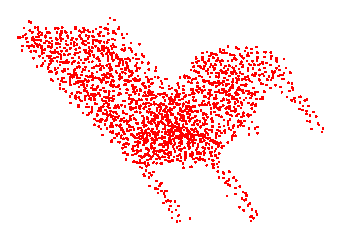
\includegraphics[scale=0.5]{pc2_example}};
				\node at (2.5,0) {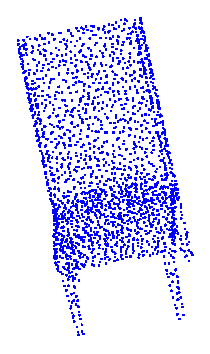
\includegraphics[scale=0.5]{pc1_example}};
				\node at (4.0,0) {\large $\xrightarrow{T\in\SE{3}}$};
				\node at (5.5,0) {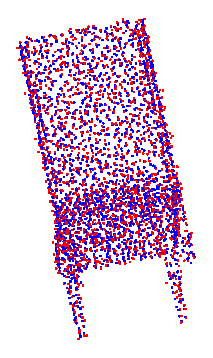
\includegraphics[scale=0.5]{pc12_example}};
				
				\node at (0,-1.8) {\footnotesize $\{p_i\in\mathbb{R}^3\}$};
				\node at (2.7,-1.8) {\footnotesize $\{p'_i\in\mathbb{R}^3\}$};
				\node at (5.7,-1.8) {\footnotesize Align $\{p_i\}$ and $\{p'_i\}$};
				\node at (5.7,-2.2) {\footnotesize using $T\in\SE{3}$};
			\end{tikzpicture}
		}
		
		\only<2>{
			\begin{itemize}
				\item map point set: landmark/feature coordinates $\{p_i\}_{i=1}^N$ in inertial frame.
				
				\begin{itemize}
					\item Without noise: $\{p_i\}_{i=1}^N$ are deterministic.
					\item With noise: $p_i \sim \mathcal{N}(\bar{p}_i, B_i)$.
				\end{itemize}
			
				\item measurement point set: coordinates in body-fixed frame.
				
				\centerline{
					\begin{beamercolorbox}[wd=10cm,sep=0.0cm,center,rounded=true,shadow=true]{numerical}
						\footnotesize
						\vspace{-0.3cm}
						\begin{align*}
							p'_i = R^T(p_i-t) + \mathcal{N}(0,A_i).
						\end{align*}
						\vspace{-0.4cm}
					\end{beamercolorbox}
				}
			
				\item The correspondences between two point sets are known.
			
				\item Objective: find the distribution of $(R,t)\in\SE{3}$, and match it to an MFG.
			\end{itemize}
		}
	\end{itemize}
\end{frame}

\begin{frame}
	\frametitle{Deterministic Map Points}
	
	\begin{itemize}
		\item Likelihood for $(R,t)$
		
		\centerline{
			\begin{beamercolorbox}[wd=10cm,sep=0.0cm,center,rounded=true,shadow=true]{numerical}
				\footnotesize
				\vspace{-0.3cm}
				\begin{align*}
					p(p'_1,\ldots,p'_N | R,t) = \expb{ -\frac{1}{2} \sum_{i=1}^N \big(R^T(p_i-t)-p'_i\big)^T A_i^{-1} \big(R^T(p_i-t)-p'_i\big) }.
				\end{align*}
				\vspace{-0.3cm}
			\end{beamercolorbox}
		}
	
		\vspace{0.2cm}
		\item Factorization of Likelihood
		
		\centerline{
			\begin{beamercolorbox}[wd=10cm,sep=0.0cm,center,rounded=true,shadow=true]{numerical}
				\footnotesize
				\vspace{-0.3cm}
				\begin{align*}
					p(p'_1,\ldots,p'_N | R,t) &\propto p_R(R) p_{t|R}(t|R), \\
					p_R(R) &= \expb{-\tfrac{1}{2} (\mathbf{T}\bm{p}'-\mathbf{T}\bm{p}_m)^T \big(\mathbf{T}\mathbf{A}\mathbf{T}^T\big)^{-1} (\mathbf{T}\bm{p}'-\mathbf{T}\bm{p}_m)}, \\
					p_{t|R}(t|R) &= \expb{-\tfrac{1}{2} (t - \mu_{t|R})^T \Sigma_{t|R}^{-1} (t - \mu_{t|R})}.
				\end{align*}
				\vspace{-0.4cm}
			\end{beamercolorbox}
		}
	
		\begin{itemize}
			\item Motivated by the conventional SVD method.
			\item $\mathbf{T}\bm{p}_m$ is independent of $t$.
			\item If $A_i = \sigma_i^2I_{3\times 3}$, $\Sigma_{t|R}$ is independent of $R$, $\mu_{t|R}$ is linear in $R$.
			\item Use \Emph{marginal MLE} to $p_R(R)$.
			\item Use \Emph{conditional MLE} to $p_{x|R}(x|R)$.
		\end{itemize}
	\end{itemize}
\end{frame}

\begin{frame}
	\frametitle{Marginal MLE}
	
	\begin{itemize}
		\item Marginal MLE for $p_R(R)$
		
		\centerline{
			\begin{beamercolorbox}[wd=10cm,sep=0.0cm,center,rounded=true,shadow=true]{numerical}
				\footnotesize
				\vspace{-0.3cm}
				\begin{align*}
					p_R(R) &= \expb{-\tfrac{1}{2} (\mathbf{T}\bm{p}'-\mathbf{T}\bm{p}_m)^T \big(\mathbf{T}\mathbf{A}\mathbf{T}^T\big)^{-1} (\mathbf{T}\bm{p}'-\mathbf{T}\bm{p}_m)}
				\end{align*}
				\vspace{-0.4cm}
			\end{beamercolorbox}
		}
	
		\begin{itemize}
			\item $\mathbf{T}$ is used to center $\{p_i\}$ and $\{p'_i\}$, $i=1,\ldots,N-1$.
			
			\centerline{
				\begin{beamercolorbox}[wd=10cm,sep=0.0cm,center,rounded=true,shadow=true]{numerical}
					\footnotesize
					\vspace{-0.3cm}
					\begin{align*}
						q_i = p_i-\frac{1}{N} \sum_{i=1}^N p_i, \qquad\qquad q'_i = p'_i - \frac{1}{N} \sum_{i=1}^N p'_i = R^Tq_i + \text{noise},
					\end{align*}
					\vspace{-0.3cm}
				\end{beamercolorbox}
			}
		
			\item Wahba's problem:
			\begin{itemize}
				\item $\{q_i\}_{i=1}^{N-1}$ are reference vectors in the inertial frame.
				\item $\{q'_i\}_{i=1}^{N-1}$ are measurements in the body-fixed frame.
				\item However, $\{q'_i\}$ are \Emph{correlated}.
			\end{itemize}
		
			\item \Emph{Importance sampling}
			\begin{itemize}
				\item Find a matrix Fisher distribution $\mathcal{M}(F)$ through Wahba's problem.
				\item Select sigma points $\{R_i,w_i\}_{i=1}^7$ from $\mathcal{M}(F)$.
				\item Reweigh the weights as $w_i^+ = w_i p_R(R_i) / p_\text{prop}(R_i)$.
				\item Use MLE to the reweighed sigma points $\{R_i,w_i^+\}_{i=1}^7$.
				\item Progressive update can also be applied to improve accuracy.
			\end{itemize}
		\end{itemize}
	\end{itemize}
\end{frame}

\begin{frame}
	\frametitle{Simulation: KL-Divergence}
	
	\begin{itemize}
		\item Comparison with LM-Optimization
		\begin{itemize}
			\item Find the best $(R,t)\in\SE{3}$ that maximizes the likelihood $p(p'_i,\ldots,p'_N|R,t)$.
			
			\item Gradient based Gauss-Newton method for nonlinear least square.
			
			\item The Jacobian $(J_r^TJ_r)^{-1} \in \mathbb{R}^{6\times 6}$ represents the covariance matrix. 
		\end{itemize}
	
		\vspace{0.1cm}
		\item KL-Divergence
		\begin{itemize}
			\item A metric for the difference between two probability distributions.
			
			\item Simulation results with varying number of map points.
			
			\vspace{0.1cm}
			\centerline{
				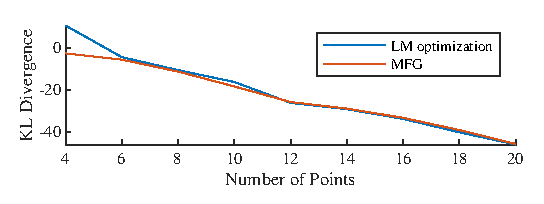
\includegraphics[scale=0.7]{VIO-KL}
			}
		
			\vspace{0.1cm}
			\item The MFG is a much \Emph{better approximation} of the true likelihood when the number of map points is small, i.e., the \Emph{uncertainty is large}.
		\end{itemize}
	\end{itemize}
\end{frame}

\begin{frame}
	\frametitle{Simulation: Pose Accuracy}
	
	\begin{center}
		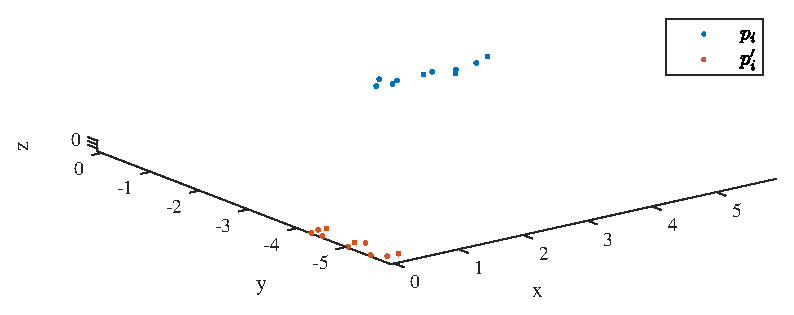
\includegraphics[scale=0.5]{pointSets}
	\end{center}

	\only<1>{
		\begin{itemize}
			\item Two Point Sets Alignment
			\begin{itemize}
				\item Ten map points scattered around $x$-axis.
				\item \Emph{The uncertainty in $x$-axis in inertial frame is large}.
				\item The uncertainties in two other axes are small.
				\item Concentration of map points around $x$-axis, $a\in\{1,0.1,0.01,0\}$.
			\end{itemize}
		\end{itemize}
	}

	\only<2>{
		\begin{itemize}
			\item Estimation Errors
			
			\vspace{0.2cm}
			\begin{center}
				\scriptsize
				\begin{tabular}{l|cccc}
					\hline\hline
					estimator & \multicolumn{4}{c}{MFG} \\ \hline
					a & 1 & 0.1 & 0.01 & 0 \\ \hline
					att err (deg) & 3.93$\pm$1.79 & 24.0$\pm$21.7 & 82.4$\pm$51.4 & 90.1$\pm$0.2 \\
					pos err & 0.28$\pm$0.15 & \Emph{0.36$\pm$0.20} & \Emph{0.14$\pm$0.06} & \Emph{0.11$\pm$0.08} \\
					\midrule[1.2pt]
					estimator & \multicolumn{4}{c}{LM optimization} \\ \hline
					a & 1 & 0.1 & 0.01 & 0 \\ \hline
					att err (deg) & 3.93$\pm$1.79 & 24.0$\pm$21.8 & 80.7$\pm$51.2 & 90.1$\pm$0.1 \\
					pos err & 0.28$\pm$0.15 & \Emph{0.39$\pm$0.22} & \Emph{0.39$\pm$0.22} & \Emph{0.38$\pm$0.20} \\
					\hline\hline
				\end{tabular}
			\end{center}
		
			\begin{itemize}
				\item MFG has \Emph{better accuracy} in translation when the \Emph{uncertainty about $x$-axis is large}.
			\end{itemize}
		\end{itemize}
	}
\end{frame}

\begin{frame}
	\frametitle{Simulation: Visual-Inertial Navigation}
	
	\begin{itemize}
		\item Bayesian Assumed Density Filter
		\begin{itemize}
			\item Uncertainty propagation: IMU kinematics.
			\item Measurement update: landmark coordinate measurements combined with pose prior.
		\end{itemize}
	
		\only<1>{
			\item Settings
			\begin{itemize}
				\item A circular trajectory with landmarks scattered around.
				
				\vspace{0.2cm}
				\centerline{
					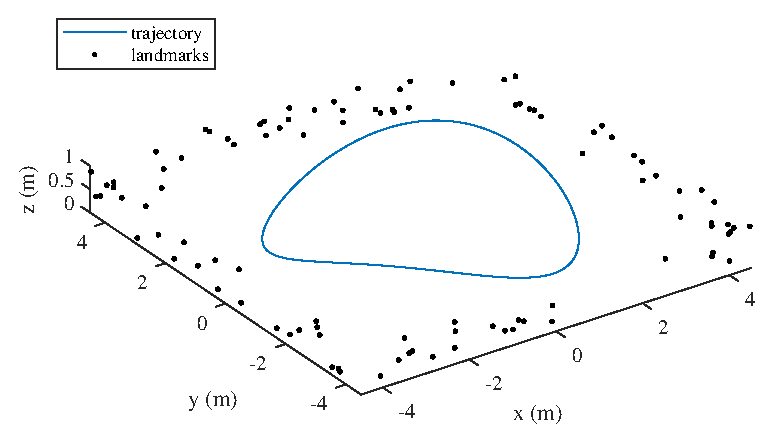
\includegraphics[scale=0.5]{VIO-trajectory}
				}
				
				\item Initial conditions: \Emph{reversed yaw direction}.
			\end{itemize}
		}
		
		\only<2>{
			\item Estimation Errors
			
			\vspace{0.2cm}
			\centerline{
				\includegraphics[scale=0.6]{VIO-NoMap-trajectory}
			}
		}
	
		\only<3>{
			\vspace{0.2cm}
			\item Estimation Errors
			\begin{itemize}
				\item MFG has \Emph{Faster convergence} of yaw.
				\item MFG has \Emph{Better accuracy} of position and velocity.
			\end{itemize}
			
			\vspace{0.2cm}
			\centerline{
				\includegraphics[scale=0.6]{VIO-NoMap-error}
			}
		}
	\end{itemize}
\end{frame}

\begin{frame}
	\frametitle{Noisy Map Points}
	
	\begin{itemize}
		\item Posterior Density for Pose $(R,t)$ and Map Points $\{p_i\}$
		
		\centerline{
			\begin{beamercolorbox}[wd=10cm,sep=0.0cm,center,rounded=true,shadow=true]{numerical}
				\footnotesize
				\vspace{-0.3cm}
				\begin{align*}
					p\left( R,t,\{p_i\} | \{p'_i\} \right) &\propto \expb{-\frac{1}{2} \sum_{i=1}^{N} \big(R^T(p_i-t)-p'_i\big)^T A_i^{-1} \big(R^T(p_i-t)-p'_i\big)} \nonumber \\
					&\qquad\qquad \cdot \expb{-\frac{1}{2}\sum_{i=1}^N (p_i-\bar{p}_i)^T B_i^{-1} (p_i-\bar{p}_i)}.
				\end{align*}
				\vspace{-0.3cm}
			\end{beamercolorbox}
		}
		
		\item Factorization of Posterior Density
		
		\centerline{
			\begin{beamercolorbox}[wd=10cm,sep=0.0cm,center,rounded=true,shadow=true]{numerical}
				\footnotesize
				\vspace{-0.3cm}
				\begin{align*}
					p\left( R,t,\{p_i\} | \{p'_i\} \right) &\propto p_R(R|\{p'_i\}) \cdot p_{x|R}(x|R), \\
					p_R(R) &= \expb{-\tfrac{1}{2} (\mathbf{T}\bm{p}'-\mathbf{T}\bm{p}_m)^T \big(\mathbf{T}\mathbf{A}\mathbf{T}^T\big)^{-1} (\mathbf{T}\bm{p}'-\mathbf{T}\bm{p}_m)}, \\
					p_{x|R}(x|R) &= \expb{-\tfrac{1}{2} (x - \mu_{x|R})^T \Sigma_{x|R}^{-1} (x - \mu_{x|R})}.
				\end{align*}
				\vspace{-0.3cm}
			\end{beamercolorbox}
		}
	
		\begin{itemize}
			\item $x = [t, p_1, \ldots, p_N]$ is the translation and all map points.
			
			\item Use marginal MLE to $p_R(R)$.
			
			\item Use conditional MLE to $p_{x|R}(x|R)$ with $\{p_i\}$ marginalized.
			
			\item Calculate $\expect{p_i}$, $\expect{p_ip_i^T}$, and match them to Gaussian distributions.
		\end{itemize}
	\end{itemize}
\end{frame}

\begin{frame}
	\frametitle{Simulation: Pose and Map Accuracy}
	
	\begin{itemize}
		\item Two Point Sets Alignment
		\begin{itemize}
			\item Ten map points:
			\begin{itemize}
				\item $N_1$ of them have small uncertainty.
				\item The rest of $10-N_1$ have large uncertainty.
			\end{itemize}
		\end{itemize}
	
		\item Estimation Accuracy
		
		\vspace{0.2cm}
		\centerline{
			\scriptsize
			\begin{tabular}{l|ccc}
				\hline\hline
				estimator & \multicolumn{3}{c}{MFG} \\ \hline
				$N_1$ & 4 & 2 & 0 \\ \hline
				att err (deg) & \color{red} 16.5$\pm$7.9 & \color{red} 50.6$\pm$30.9 & 77.1$\pm$41.1 \\
				pos err & 0.305$\pm$0.147 & 0.755$\pm$0.372 & \Emph{1.05$\pm$0.38} \\
				map err ($N_1$) & 0.138$\pm$0.030& 0.149$\pm$0.046 & - \\
				map err ($10-N_1$) & \Emph{0.225$\pm$0.056} & \Emph{0.501$\pm$0.189} & \Emph{0.661$\pm$0.173} \\
				\midrule[1.2pt]
				estimator & \multicolumn{3}{c}{LM optimization} \\ \hline
				$N_1$ & 4 & 2 & 0 \\ \hline
				att err (deg) & \color{red} 16.0$\pm$7.5 & \color{red} 48.6$\pm$29.5 & 76.4$\pm$40.8 \\
				pos err & 0.294$\pm$0.149 & 0.772$\pm$0.455 & \Emph{1.17$\pm$0.55} \\
				map err ($N_1$) & 0.138$\pm$0.030 & 0.153$\pm$0.048 & - \\
				map err ($10-N_1$) & \Emph{0.230$\pm$0.056} & \Emph{0.518$\pm$0.216} & \Emph{0.708$\pm$0.196} \\
				\hline\hline
			\end{tabular}
		}
	\end{itemize}
\end{frame}

\begin{frame}
	\frametitle{Simulation: Visual-Inertial Navigation}
	
	\begin{itemize}
		\item Bayesian Assumed Density Filter
		\begin{itemize}
			\item Uncertainty propagation: IMU kinematics, static map points.
			\item Measurement update: landmark coordinate measurements combined with pose and map priors.
		\end{itemize}
	
		\vspace{0.1cm}
		\item Initial conditions: \Emph{reversed yaw direction}.
		
		\only<1>{
			\item Estimation Errors
			
			\vspace{0.1cm}
			\centerline{
				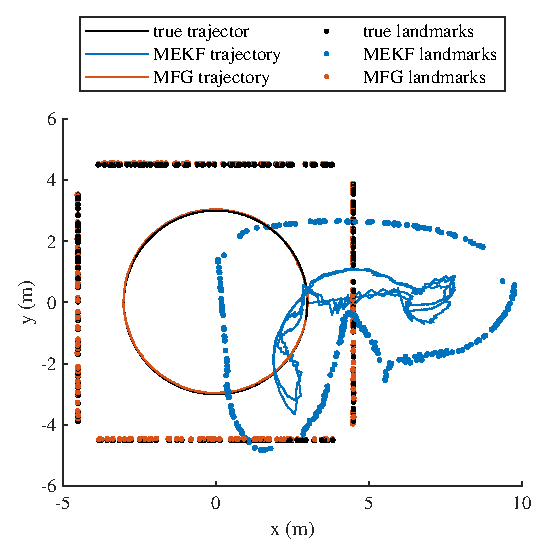
\includegraphics[scale=0.7]{VIO-map-filter-trajectory1}
			}
		}
		
		\only<2>{
			\vspace{0.1cm}
			\item Estimation Errors
			\begin{itemize}
				\item MFG \Emph{converges very quickly} from wrong initial attitude
				\item MEKF \Emph{does not converge}.
			\end{itemize}
			
			\vspace{0.2cm}
			\centerline{
				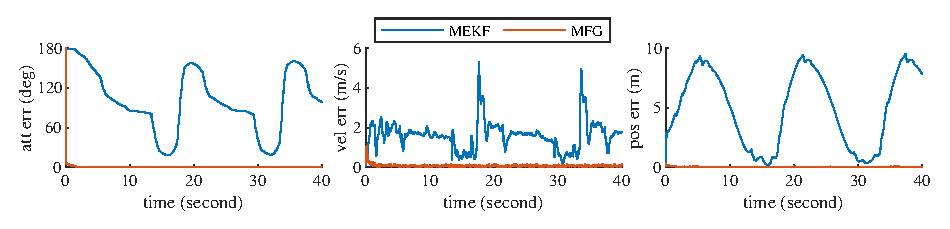
\includegraphics[scale=0.6]{VIO-Map-error}
			}
		}
	\end{itemize}
\end{frame}

\begin{frame}
	\frametitle{Visual-Inertial Odometry}
	
	\begin{itemize}
		\item No Prior Information for the Map
		\begin{itemize}
			\item The features captured by cameras are usually geometric corners.
			\item The map must be built incrementally from previously captured corners.
		\end{itemize}
	
		\vspace{0.2cm}
		\item Build Map From Feature Coordinate Measurements
		
		\centerline{
			\begin{beamercolorbox}[wd=10cm,sep=0.0cm,center,rounded=true,shadow=true]{numerical}
				\footnotesize
				\vspace{-0.3cm}
				\begin{align*}
					p_{p_i}(p_i) = \int_{R\in\SO{3}} \int_{t\in\mathbb{R}^3} p_{R,t}(R,t) p_{p'_i}\left( R^T(p_i-t) \right) \diff t \diff R.
				\end{align*}
				\vspace{-0.3cm}
			\end{beamercolorbox}
		}
		
		\begin{itemize}
			\item $p_{R,t}(R,t)$ is the probability density for pose.
			\item $p_{p'_i}(p'_i)$ is the probability density for measurements.
			\item Calculate $\expect{p_i}$, $\expect{p_ip_i^T}$, and match them to Gaussian distributions.
			\item When $R$ has large uncertainty, $p_{p_i}(p_i)$ is far from a Gaussian distribution, so this method is \Emph{not suitable for large uncertainty}.
		\end{itemize}
	\end{itemize}
\end{frame}

\begin{frame}
	\frametitle{VCU-RVI Dataset}
	
	\begin{itemize}
		\item VCU-RVI Dataset: Visual-Inertial Odometry
		\begin{itemize}
			\item Inertial and RGB-D camera measurements.
			\item Ground truth provided by a motion capture system.
		\end{itemize}
	
		\vspace{0.1cm}
		\item Preliminary Results (Proof of Concept)
		
		\only<1>{
			\vspace{0.2cm}
			\centerline{
				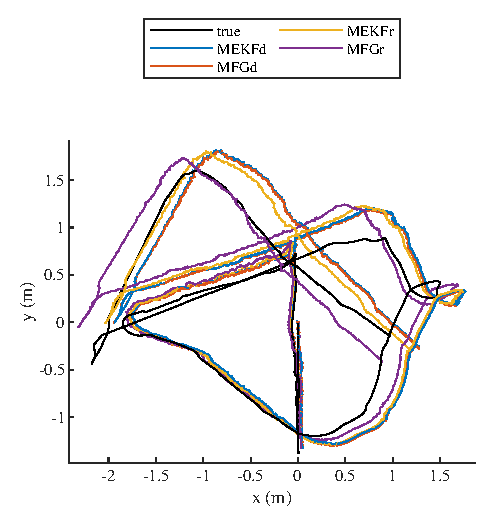
\includegraphics[scale=0.6]{VIO-VCU_RVI-trajectory1}
			}
		}
	\end{itemize}
\end{frame}

\section{Summary}

\begin{frame}
	\frametitle{Summary of Contributions}
	
	\begin{itemize}
		\item Matrix Fisher Distribution
		\begin{itemize}
			\item Recursive algorithms for higher order central moments.
			\item Highly concentrated approximates in two degrees of freedom.
		\end{itemize}
	
		\vspace{0.2cm}
		\item Matrix Fisher--Gaussian Distribution
		\begin{itemize}
			\item Construction and closed form maximum likelihood estimation.
			\item Bingham--Gaussian distribution.
		\end{itemize}
	
		\vspace{0.2cm}
		\item Application of MFG to Estimation Problems
		\begin{itemize}
			\item Attitude estimation (observability) with gyroscope and direction measurements.
			\item Loosely-coupled IMU-GNSS navigation.
			\item Visual-inertial navigation.
			\item Benefits of MFG
			\begin{itemize}
				\item Better accuracy when the attitude uncertainty is large.
				\item Faster convergence speed from wrong initial conditions.
			\end{itemize}
		\end{itemize}
	\end{itemize}
\end{frame}

\end{document}


